\chapter[Single VLQ search]{Search for a single produced \Tp~decaying into top and Higgs in the full hadronic final state}
\label{chap:search}

In the present chapter the search performed using 2012 data collected by CMS for a \Tp~in the full hadronic final state is described. The theoretical formalism for such object has been described on section~\ref{chap:VLQ}. In addition, a feasibility study for this search has been presented in chapter~\ref{chap:pheno}. As discussed in it, a resonance in the five jets invariant mass is looked for.

\section{Analysis Strategy}
\label{sec:stra}

The strategy of the analysis is based on a high signal efficiency while keeping under control the background. The main background for the hadronic final states is multijet production. This background should not present any resonance in the 5-jets invariant mass variable but purely a continuum. %In order to keep high signal efficiency while constraining background, strategy to optimize the selection is based on high signal efficiency criteria (around 80-90\%) and on multiplication of them.

Several variables to distinguish between SM backgrounds and the signal have been identified, the most important one being the number of b-tagged jets. In the signal, at least three jets coming from b-quarks are expected, and consequently, at least three b-tagged jets are expected. After requiring such condition, \ttbar~become an important background for the analysis. %The last part of the selection will be designed to diminish this background.

\section{Datasets}
\label{sec:data}

The analysis use the MultiJet primary dataset processed with the reconstruction of January 22th 2013. This reconstruction procedure is the most expensive processing of data, where all the final objects used in analyses are reconstructed. All detector information is used in the vertexing and tracking algorithms to reconstruct global objects as muons or to reconstruct jets by different algorithms with anti-kt or Cambridge-Aachen algorithms (see section~\ref{sec:jets}). A primary dataset is a set of events passing trigger selections without any further selection. They are named accordingly to their high level trigger path, in our case trigger paths requiring at least 2 jets. The processed datasets are listed in table~\ref{tab:datasets}.

\begin{table*}[htbH]
\begin{center}
\resizebox{\textwidth}{!}{
\begin{tabular}{|c|c|}
\hline 
Dataset name & Int. Luminosity ($\text{pb}^{-1}$) \\
\hline
/MultiJet/Run2012A-22Jan2013-v1/AOD & 889.4 \\
/MultiJet1Parked/Run2012B-05Nov2012-v2/AOD & 4429.0 \\
/MultiJet1Parked/Run2012C-part1-05Nov2012-v2/AOD & 494.6 \\
/MultiJet1Parked/Run2012C-part2-05Nov2012-v2/AOD & 6654.0 \\
/MultiJet1Parked/Run2012D-part1-10Dec2012-v1/AOD & 5955.1 \\
/MultiJet1Parked/Run2012D-part2-17Jan2013-v1/AOD & 734.0 \\
/MultiJet1Parked/Run2012D-part2-PixelRecover-17Jan2013-v1 & 538.4 \\
\hline
\multicolumn{1}{|r|}{\textit{Total}} & 19694.5 \\
\hline
\end{tabular}
}
\caption{List of Multijet Primary Dataset used in the analysis and the corresponding integrated luminosity calculated using the golden JSON (Java Script Object Notation) file. The golden JSON file contains the information about the luminosity sections considered as good for all runs. A good luminosity section is defined as a luminosity section where the detector was fully functioning, this is all subsystems were taking data and without problems.  \label{tab:datasets}}
\end{center}
\end{table*}

In addition, the MC samples processed to study the different backgrounds entering the analysis are presented in table~\ref{tab:MCbkg}. QCD, in \pt~hat (for initial partons \pt~ranges), and diboson samples have been generated using Pythia 6~\cite{Sjostrand:2006za}, while the ones in \HT~bins were generated with MadGraph 5~\cite{Alwall:2014hca, Alwall:2011uj} interfaced with Pythia 6. The same generators were used to generate \ttbar~MC samples with the additional usage of MadSpin~\cite{Artoisenet:2012st, Frixione:2007zp}. The single top samples were generated using Powheg~\cite{Nason:2004rx, Frixione:2007vw, Alioli:2010xd} generator. 

\begin{table*}[htbH]
\begin{center}
\resizebox{\textwidth}{!}{
\begin{tabular}{|c|c|c|}
\hline 
Samples & Cross-Section (pb) & Number of events\\
\hline
QCD\_Pt-120to170\_TuneZ2star\_8TeV\_pythia6 & 16\(\times 10^4\) & 5.9M\\
QCD\_Pt-170to300\_TuneZ2star\_8TeV\_pythia6 & 34\(\times 10^3\) & 5.8M\\
QCD\_Pt-300to470\_TuneZ2star\_8TeV\_pythia6 & 18\(\times 10^2\) & 5.9M\\ 
QCD\_Pt-470to600\_TuneZ2star\_8TeV\_pythia6 & 114 & 3.9M\\
QCD\_Pt-600to800\_TuneZ2star\_8TeV\_pythia6 & 27 & 3.9M\\
QCD\_Pt-800to1000\_TuneZ2star\_8TeV\_pythia6 & 3.5 & 3.9M\\
QCD\_HT-500To1000\_TuneZ2star\_8TeV-madgraph-pythia6 & 84\(\times 10^2\) & 30M\\ 
QCD\_HT-1000ToInf\_TuneZ2star\_8TeV-madgraph-pythia6 & 2\(\times 10^2\) & 14M\\ 
DYToCC\_M\_50\_TuneZ2star\_8TeV\_pythia6 & 31\(\times 10^2\) & 2M\\
DYToBB\_M\_50\_TuneZ2star\_8TeV\_pythia6 & 38\(\times 10^2\) & 2M\\
TTJets\_MSDecays\_central\_TuneZ2star\_8TeV-madgraph-tauola & 247.7 [NNLO] & 62M\\
%TT\_CT10\_TuneZ2star\_8TeV-powheg-tauola & 247.7 [NNLO] & 22M\\
T\_tW-channel-DR\_TuneZ2star\_8TeV-powheg-tauola & 11.1 [NNLO] &497k\\
T\_s-channel\_TuneZ2star\_8TeV-powheg-tauola & 3.79 [NNLO] & 260k\\
T\_t-channel\_TuneZ2star\_8TeV-powheg-tauola & 54.9 [NNLO] & 3.7M\\
Tbar\_tW-channel-DR\_TuneZ2star\_8TeV-powheg-tauola & 11.1 [NNLO] & 493k\\
Tbar\_s-channel\_TuneZ2star\_8TeV-powheg-tauola & 1.76 [NNLO] & 140k\\
Tbar\_t-channel\_TuneZ2star\_8TeV-powheg-tauola & 29.7 [NNLO] & 1.9M\\
WZ\_TuneZ2star\_8TeV\_pythia6\_tauola & 33.6 [NLO] & 10M\\
ZZ\_TuneZ2star\_8TeV\_pythia6\_tauola & 7.6 [NLO] & 9.8M\\
WW\_TuneZ2star\_8TeV\_pythia6\_tauola & 56 [NLO] & 10M\\
TTH\_Inclusive\_M-125\_8TeV\_pythia6 & 0.13 [NLO] & 100K\\
\hline
\end{tabular}
}
\caption{List of Monte-Carlo background samples used in the analysis, their corresponding cross-section and their number of events.\label{tab:MCbkg}}
\end{center}
\end{table*}

Finally, for the simulation of signal several samples for different \Tp~masses have been processed. Nine different mass points between 600 \GeVcc~and 1 TeV/$\text{c}^{2}$ in steps of 50 \GeVcc~have been utilized. The processed signal samples are shown in table~\ref{tab:MCsig}. These samples were generated with MadGraph 5 and Pythia 6.

\begin{table*}[htbH]
\begin{center}
\resizebox{\textwidth}{!}{
\begin{tabular}{|c|c|c|c|}
\hline 
Sample & \Tp~Mass & Cross-Section & Number of events\\
            & (GeV$/c^{2}$) &  (fb) & \\
\hline
TprimeJetToTH\_M-600\_TuneZ2star\_8TeV-madgraph\_tauola & 600 & 215.4 & 95K \\
TprimeJetToTH\_M-650\_TuneZ2star\_8TeV-madgraph\_tauola & 650 & 177.8 & 99K \\
TprimeJetToTH\_M-700\_TuneZ2star\_8TeV-madgraph\_tauola & 700 & 143.7 & 99K \\
TprimeJetToTH\_M-750\_TuneZ2star\_8TeV-madgraph\_tauola & 750 & 118.6 & 99K \\
TprimeJetToTH\_M-800\_TuneZ2star\_8TeV-madgraph\_tauola & 800 & 100 & 96K \\
TprimeJetToTH\_M-850\_TuneZ2star\_8TeV-madgraph\_tauola & 850 & 84.3 & 99K \\
TprimeJetToTH\_M-900\_TuneZ2star\_8TeV-madgraph\_tauola & 900 & 72.6 & 99K \\
TprimeJetToTH\_M-950\_TuneZ2star\_8TeV-madgraph\_tauola & 950 & 62.6 & 96K \\
TprimeJetToTH\_M-1000\_TuneZ2star\_8TeV-madgraph\_tauola & 1000 & 53.9 & 99K \\
\hline
\end{tabular}
}
\caption{List of Monte-Carlo signal samples used in the analysis, their corresponding cross-section and \Tp~mass.\label{tab:MCsig}}
\end{center}
\end{table*}

The signal samples have been produced with only two decay channels for the Higgs boson: \bbbar~and $\tau^{-}\tau^{+}$. Thus, in order to obtain the correct branching ratio of the Higgs to \bbbar, a rescaling factor must be applied. The branching ratio of this channel for SM Higgs of 125 GeV/$\text{c}^{2}$ is 0.57~\cite{Heinemeyer:2013tqa}. However, in signal samples the effective branching ratio is 0.94. The mass point signal samples have 94\% of times the Higgs boson decaying into \bbbar~and 6\% to $\tau^{-}\tau^{+}$. In consequence, a weight of 0.61 has been applied to these samples to obtain the correct branching ratio. %In figure~\ref{fig:BR_Higgs_SignalSamples}, it can be seen the relative content of 700 GeV/$\text{c}^{2}$ mass point into the two produced channels. Similar contents were found for all mass points. In consequence, a weight of 0.61 was considered for all signal samples.

%\begin{figure}[!Hhtbp]
%  \begin{center}
%    \includegraphics[width=0.9\textwidth]{figs/Ana/BrachingRatios_S700.png}
%    \caption{Higgs decay channels in the 700 GeV/$\text{c}^{2}$ mass point. In the figure, the x-axis represents PDG number of the particles coming from the Higgs, 5 corresponds to the b-quark and 15 to $\tau$ lepton. The histogram is normalized to unity.}
%    \label{fig:BR_Higgs_SignalSamples}
%  \end{center}
%\end{figure}

%\begin{TOINCLUDE}Table with Multijet primary datasets and integrated luminosity. Tables for MC samples, backgrounds and signal mass points.\end{TOINCLUDE}

\section{Event selection}
\label{sec:sel}

In the following sections the event processing and selection for the analysis are presented. A pre-processing of events is performed, which includes several stages to filter the events. For example, only the events in luminosity sections where the detector was working correctly, all subdetectors were on and running without problematic behavior, were selected and processed. From these pre-processed events the analysis selection is performed.

\subsection{Event processing}

As first step, data and MC events were processed with PAT (Physics Analysis Toolkit)~\cite{Adam:2010zza}, to produce PAT-tuples. PAT simplifies access to reconstructed objects and tools developed for analyses. It constitutes a common work-ground where analysts can find a simplified access to event content and to the full set of CMS tools. This step makes a first selection of objects with very basic cuts as a minimal jet $p_{T}$. Only jets within $|\eta|<5$, to cover the majority of the HCAL acceptance and include forward jets from signal, and with at least a $p_{T}$ of 20 GeV/c are considered. In addition, several noise filters are applied. For example, only events with at least one good primary vertex ($\text{n.d.o.f.} \ge 4,\; |z|<24 \;\text{cm},\; |\rho|< 2 \;\text{cm}$) are kept. In the reconstruction of primary vertices the number degrees of freedom (n.d.o.f) is related to the number of tracks associated to the vertex, $z$ is its position in the beam direction, and $\rho$ is its ``mass'', a weight assigned by the reconstruction algorithm associated to its compatibility to form a track cluster. In addition, jets by using particles reconstructed via PF algorithm~\cite{CMS:2009nxa,CMS:2010eua,CMS:2010byl,CMS:2010aua} and Charge Hadron Subtracted (CHS) technique~\cite{Kirschenmann:1627818} are corrected with the jet energy corrections (JEC, described in section~\ref{sec:JEC}). %Afterward, the PAT-tuples were dumped into a reduced ntuple format. 

An important setup for the processing of samples in CMS is the selection of the global tag. For data, it contains calibration and alignment information of the detector; and for MC, is used to mimic real detector conditions, thus to get closer MC simulations to data.

In MC samples, the pileup has to be corrected to observed pileup in data. For these samples a model to simulate expected pileup in data, called scenario, is used. The pileup scenario used for MC simulation does not describe correctly the data, therefore the MC samples have been weighted in correspondence. Figure~\ref{fig:PU_distros} shows the pileup variable for data and MC (for the scenario 10 - S10), and the weight from the ratio for each bin between data and MC. The obtained weights were applied to MC events as a function of their true number of interactions. For data, the true number of interactions represents the expected number of interactions per crossing for a given lumi section from the average bunch instantaneous luminosity with respect to the total inelastic cross section.

\begin{figure}[!Hhtbp]
  \begin{center}
    \includegraphics[width=0.49\textwidth]{figs/Ana/DataPU40.png}
    \includegraphics[width=0.49\textwidth]{figs/Ana/MCPU40.png}
    \includegraphics[width=0.5\textwidth]{figs/Ana/WeightPU40.png}
    \caption{Pileup for data [up-left], MC S10 [up-right] and ratio between them [bottom].}
    \label{fig:PU_distros}
  \end{center}
\end{figure}

To check the correctness of the procedure, the number of vertices in data and MC were compared. This comparison can be found in figure~\ref{fig:NV_dataMC}, and it is performed before cutting on number of b-tagged jets. After this reweighting procedure, the sum of MC samples correctly describe data number of vertices.

\begin{figure}[!Hhtbp]
  \begin{center}
    \includegraphics[width=0.8\textwidth]{figs/Ana/Nvtcs.png}
    \caption{Number of vertices distribution for data and MC samples. The comparison has been performed after basic selection except number of b-tagged jets (the basic selection is described in the next section,~\ref{sec:basicsel}). The gray band correspond to the statistical error of MC samples sum. Normalization of MC samples was done to the 19.7~fb$^{-1}$.}
    \label{fig:NV_dataMC}
  \end{center}
\end{figure}

\subsection{Basic selection}
\label{sec:basicsel}

The selection starts with the trigger requirement. The level 1 trigger selects multijet events with at least 4 central jets (\etal{3}) with a \ptg{32}~or \ptg{36}~or \ptg{40}, or events with at least two central jets with \ptg{52}~or \ptg{56}~or \ptg{64}, or events with \HTg{125}~or \HTg{150}~or \HTg{175} with at least 4 central jets. To obtain a fully unprescaled trigger selection, on top of the loosest trigger requirement that is prescaled, tighter unprescaled trigger requirements were added. The HLT path chosen require at least 6 jets with a \ptg{20}, 4 with a \ptg{60} and two with a \ptg{80}. These jets are required to have \etal{3}. This HLT path is named \textit{DiJet\_80\_DiJet\_60\_DiJet\_20}. The HLT works with CaloJets, jets reconstructed with calorimeter information, slightly different from PF jets from final event reconstruction. Right after the requirement from the trigger, a first cut is applied, to close up selection to the parameter space of the trigger selection. Only events with two jets with \ptg{90}, two jets with \ptg{70} and two jets with \ptg{30} were kept. This selection is applied over PF jets. %In these first cuts no requirement on the $\eta$ of jets was applied.

As a second selection step, at least 5 jets with \ptg{30} and \etal{2.5} and at least one additional jet with \ptg{30} and \etal{5} were required for all events. This cut is driven by signal properties. The \Tp~is produced in association with a light jet, that is produced in the forward $\eta$ region. In addition, the \Tp~decay products (5 jets in the full hadronic final state) are essentially produced in the tracker acceptance (\etal{2.5}). Figure~\ref{fig:SixthJetTp} shows the $\eta$ distribution of the accompanying jet from signal MC sample with M=700 \GeVcc~using MC truth information. At this stage of the selection all events have at least 6 jets with \ptg{30}. %, and the other jets are required to have a \ptg{20}. %We will refer to this first part as the acceptance selection.

\begin{figure}[!Hhtbp]
  \begin{center}
    \includegraphics[width=0.8\textwidth]{figs/Ana/SixthJetMCTruth.png}
    \caption{Distribution of pseudorapidity of the accompanying jet produced with the \Tp. The distribution is taken from the signal MC sample with M=700 \GeVcc~and it is normalized to unity.}
    \label{fig:SixthJetTp}
  \end{center}
\end{figure}

Moreover the leading jet was required to have a \ptg{150}. With this cut \ttbar~is reduced by 32\% and QCD by 24\% (estimation performed from MC samples shown in table~\ref{tab:MCbkg}), while signal (M=700~\GeVcc) is only reduced by 9\%. As the leading jet in signal events is coming from a heavy \Tp, it is expected to have higher \pt~than in SM background events. In figure~\ref{fig:6jpt} and~\ref{fig:6jeta} the \pt~and $\eta$ of the 6 leading jets for data and MC are shown. The comparison is performed before selecting on the number of b-tagged jets. Some disagreements between MC samples and the data are expected at very high jet \pt, because QCD MC samples were processed for a \pt~up to 1000~GeV/c (see table~\ref{tab:MCbkg}). The MC samples are used in this analysis only for illustration purposes, as final background estimation has been derived directly from data. Additionally, in the $\eta$ distributions of jets a disagreement between data and MC is visible for \etag{3}. This disagreement is caused by the simulation of the trigger on MC, that do not correspond exactly with the behavior of real trigger in data. This mismatch of the trigger in MC is a motivations to estimate backgrounds from data instead of using MC. 

\begin{figure}[!Hhtbp]
  \begin{center}
    \includegraphics[width=0.4\textwidth]{figs/Ana/jet1pt.png}
    \includegraphics[width=0.4\textwidth]{figs/Ana/jet2pt.png}
    \includegraphics[width=0.4\textwidth]{figs/Ana/jet3pt.png}
    \includegraphics[width=0.4\textwidth]{figs/Ana/jet4pt.png}
    \includegraphics[width=0.4\textwidth]{figs/Ana/jet5pt.png}
    \includegraphics[width=0.4\textwidth]{figs/Ana/jet6pt.png}
    \caption{Distribution of transverse momentum of the 6 leading jets. The gray band represents the statistical uncertainties from the sum of the MC background. Reasonable agreement is observed, with the multijet process as the dominant process at this stage. Normalization of samples was done to the 19.7~fb$^{-1}$.}
    \label{fig:6jpt}
  \end{center}
\end{figure}

\begin{figure}[!Hhtbp]
  \begin{center}
    \includegraphics[width=0.4\textwidth]{figs/Ana/jet1eta.png}
    \includegraphics[width=0.4\textwidth]{figs/Ana/jet2eta.png}
    \includegraphics[width=0.4\textwidth]{figs/Ana/jet3eta.png}
    \includegraphics[width=0.4\textwidth]{figs/Ana/jet4eta.png}
    \includegraphics[width=0.4\textwidth]{figs/Ana/jet5eta.png}
    \includegraphics[width=0.4\textwidth]{figs/Ana/jet6eta.png}
    \caption{Distribution of $\eta$ of the 6 leading jets. The gray band represents the statistical uncertainties from the sum of the MC background. Reasonable agreement is observed, with the multijet process as the dominant process at this stage. Normalization of samples was done to luminosity.}
    \label{fig:6jeta}
  \end{center}
\end{figure}

After the cut on the leading jet \pt, \HTg{550} was required. Multijet background events have smaller \HT~than signal events. \HT~distribution for data and MC samples is shown in figure~\ref{fig:HT}, comparison performed before b-tagged jets multiplicity criterion. The QCD MC samples were combined to increase the statistics on this process. The QCD \HT~binned and \pt~hat samples were normalized to half the luminosity observed in the data. The combination of these samples should then correctly represent the expected multijet background for an \HTg{550}. However, as \pt~hat samples were processed only up to 1000~GeV/c some disagreement is expected at high \HT.

\begin{figure}[!Hhtbp]
  \begin{center}
    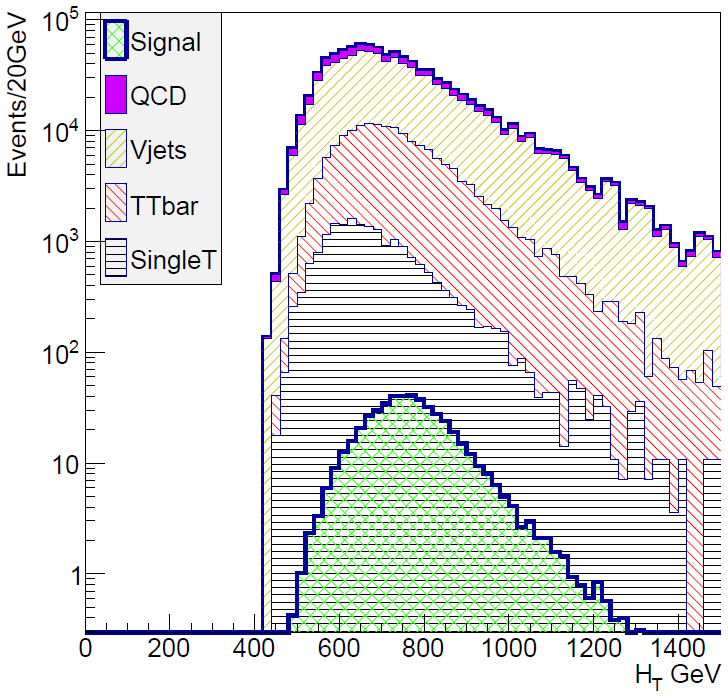
\includegraphics[width=0.8\textwidth]{figs/Ana/HT.png}
    \caption{Distribution of the $H_{T}$ variable for data and the sum of the MC samples normalized to luminosity. The signal sample (M=700 \GeVcc) is over-imposed on top of the stack of the MC samples. The gray band represents the statistical uncertainties from the sum of the MC background. Reasonable agreement is observed, with the multijet process as the dominant process at this stage. Normalization of samples was done to luminosity.}
    \label{fig:HT}
  \end{center}
\end{figure}

The final cut of the basic selection concerns the request of a minimum number of b-tagged jets. The CSV algorithm (described in section~\ref{sec:bid}) was used to identify jets coming from a b quark. In the following, b-tagged jets are defined as jets that were b-tagged by the CSV algorithm and b-jets as jets matched at generator level as coming from a b-quark (from matrix element). The medium working point was chosen as it allows to have a high efficiency on b-jet identification (70\%) with a low rate from c-quark (20\%) and light quarks (1\%)~\cite{Chatrchyan:2012jua, CMS-PAS-BTV-13-001}. In the full hadronic final state, the \Tp~decays in three b-quarks, a \bbbar~system coming from the Higgs boson and an additional b-quark from the t-quark, and two light jets from the \W~boson produced by the top. Accordingly, signal events are expected to have at least 3 b-tagged jets, while \ttbar~and QCD events should have mainly 2. QCD events can have also 4 b-tagged jets but in smaller proportion.

In principle several working points can be used to establish the b-tagged jets content of events. For the CSV algorithm three working points have been defined as function of the cut made on the discriminator value, 0.244 for the loose working point (CSVL), 0.679 for the medium (CSVM) and 0.898 for the tight working point (CSVT). For example, events can be required to have at least 3 b-tagged jets one with tight working point and two with medium working point. All possible combinations have been studied from the three available working points (loose (CSVL), medium (CSVM) and tight (CSVT)) to require at least 3 CSV b-tagged jets in order to establish which combination gave the best $S/B$ while keeping the most of signal events. For the study, the $M=700$ \GeVcc~signal sample has been used as signal and as backgrounds the \ttbar, QCD\_HT-500To1000 and QCD\_HT-1000ToInf MC samples have been utilized. The study was performed applying the basic selection, after \HT~cut. The results of the study are contained in table~\ref{tab:BCutStudy}. This table shows that the most efficient cuts to discriminate signal from backgrounds and to keep signal are to require at least 3 CSVM b-tagged jets or to require at least 2 CSVM and 1 CSVT b-tagged jets. Selecting at least 3 CSVM b-tagged jets has the same $S/B$ and $S/\sqrt{S+B}$ than requiring at least 2 CSVM and 1 CSVT b-tagged jets. However, the 3 CSVM criterion has a higher efficiency on signal. Thus, the 3 CSVM requirement is preferred over the other combinations. %For simplicity of the reconstruction procedure and the background estimation, at least 3 CSVM b-tagged jets are required. At this stage it is extremely important to keep enough signal, because the next step of the analysis involves the reconstruction of the \Tp.

\begin{table}[htbH]
\begin{center}
\resizebox{\textwidth}{!}{
\begin{tabular}{| c || c | c | c | c | c | c |}
\hline 
\textit{At least} & $\epsilon(S)$ [\%] & $\epsilon(t\bar{t})$ [\%] & $\epsilon(\text{QCD\_HT-500To1000})$ [\%] & $\epsilon(\text{QCD\_HT-1000ToInf})$ [\%] & $\frac{S}{B}\times 10^{3}$ & $\frac{S}{\sqrt{S+B}}\times 10^{2}$ \\
\hline
3 CSVL                       & $65 \pm 0.4$  & $38 \pm 0.04$  & $6 \pm 0.02$    & $7 \pm 0.02$     & $0.4 \pm 0.005$  & $24.8 \pm 0.3$ \\
3 CSVM                       & $31 \pm 0.4$  & $8 \pm 0.02$   & $1 \pm 0.01$    & $0.6 \pm 0.01$   & $1.8 \pm 0.05$   & $38.2 \pm 0.8$ \\
1 CSVL and 2 CSVM            & $55 \pm 0.4$  & $27 \pm 0.03$  & $2 \pm 0.01$    & $2 \pm 0.01$     & $0.8 \pm 0.01$   & $33.7 \pm 0.5$ \\
2 CSVL and 1 CSVM            & $64 \pm 0.4$  & $37 \pm 0.04$  & $5 \pm 0.02$    & $5 \pm 0.02$     & $0.5 \pm 0.007$  & $28.3 \pm 0.3$  \\
2 CSVM and 1 CSVT            & $29 \pm 0.4$  & $8 \pm 0.02$   & $0.5 \pm 0.006$ & $0.5 \pm 0.006$  & $1.9 \pm 0.05$   & $38.4 \pm 0.8$  \\
1 CSVM and 2 CSVT            & $22 \pm 0.4$  & $5 \pm 0.02$   & $0.3 \pm 0.005$ & $0.3 \pm 0.003$  & $2.2 \pm 0.07$   & $35.8 \pm 0.9$  \\
3 CSVT                       & $9 \pm 0.2$   & $1 \pm 0.01$   & $0.1 \pm 0.003$ & $0.09 \pm 0.002$ & $3.1 \pm 0.2$    & $27.3 \pm 1.1$  \\
1 CSVL and 2 CSVT            & $33 \pm 0.4$  & $13 \pm 0.03$  & $0.9 \pm 0.01$  & $0.8 \pm 0.007$  & $1.1 \pm 0.03$   & $31.5 \pm 0.6$  \\
2 CSVL and 1 CSVT            & $57 \pm 0.4$  & $30 \pm 0.03$  & $3 \pm 0.02$    & $3 \pm 0.01$     & $0.7 \pm 0.01$   & $31.5 \pm 0.4$  \\
1 CSVL and 1 CSVM and 1 CSVT &  $51 \pm 0.4$ &  $24 \pm 0.03$ & $2 \pm 0.01$    & $2 \pm 0.01$     & $0.9 \pm 0.02$   & $30.8 \pm 0.4$  \\
\hline

\hline
\end{tabular}
}
\caption{Comparative study of different possible combinations to require at least 3 b-tagged jets with CSVL, CSVM and CSVT working points. Efficiencies of cuts over signal and principal MC background samples are presented, as well as $\frac{S}{B}$ and $\frac{S}{S+B}$. High values of $\frac{S}{S+B}$ point to a good discrimination while keeping the signal efficiency high.\label{tab:BCutStudy}}
\end{center}
\end{table}

Additionally, the 2D plots linking the number of b-tagged jets in the three working points for signal after requiring $j_{1}>150$ GeV/c and $H_{T}>550$ GeV/c can be found in figure~\ref{fig:WPcorr}.

\begin{figure}[!Hhtbp]
  \begin{center}
    \includegraphics[width=0.65\textwidth, height=0.3\textheight]{figs/Ana/CSVMCSVT.png}
    \includegraphics[width=0.65\textwidth, height=0.3\textheight]{figs/Ana/CSVTCSVL.png}
    \includegraphics[width=0.65\textwidth, height=0.3\textheight]{figs/Ana/CSVMCSVL.png}
    \caption{2D plots between different b-tagging working points for signal MC sample (M=700 \GeVcc) with selection up to $H_{T}>550$ GeV/c. CSVM with CSVT [top], CSVT with CSVL [medium] and CSVM with CSVL [bottom]. Numbers in each bin correspond to the number of entries in the bin. These plots show the number of b-tagged jets in the three working points for the signal. They also show the link between the number of b-tagged jets in the different working points.}
    \label{fig:WPcorr}
  \end{center}
\end{figure}

As described in section~\ref{sec:bid}, the b-tagging is performed using a procedure where several jet variables are taken into account. It strongly depends on the ability to find displaced vertices, reason why it has been restricted to jets in $|\eta|<=2.4$. Even if the MC simulations have been tuned to be as close as possible to the real detector, differences with data remain. Therefore the b-tagging performance is different in data and in MC. Thus, a correction must be applied to MC to mimic b-tagging response on data. In general, the CSV algorithm is slightly more efficient for b-tagging b-jets in MC than in data, and b-tag more light jets as b-jets in data than in MC. To match MC to data a scale factor has been derived by the collaboration. It is defined for each jet depending on its flavor (b and c or light), \pt~and $\eta$. In equation~\ref{eq:Sfs}~\cite{CMS-PAS-BTV-13-001}, the parametrization of the scale factors for CSVM working point can be found. The functions are defined as $SF^{flavor}_{\eta}(p_{T})$.

\begin{eqnarray}
  \label{eq:Sfs}
  SF^{b\; or\; c}_{|\eta|\le 2.4}(x) & = & 0.938887 + 0.00017124x - 2.76366 \times 10^{-7}x^{2} \nonumber \\
  SF^{light}_{|\eta|\le 0.8}(x) & = & 1.07541 + 0.00231827x - 4.74249 \times 10^{-6}x^{2}  \nonumber \\
  &  & +2.70862 \times 10^{-9}x^{3} \nonumber \\
  SF^{light}_{0.8 < |\eta|\le 1.6}(x) & = & 1.05613 + 0.00114031x - 2.56066 \times 10^{-6}x^{2} \nonumber \\
  &  & + 1.67792 \times 10^{-9}x^{3} \nonumber \\
  SF^{light}_{1.6 < |\eta|\le 2.4}(x) & = & 1.05625 + 0.000487231x - 2.22792 \times 10^{-6}x^{2} \nonumber \\
  &  & + 1.70262 \times 10^{-9}x^{3}
\end{eqnarray}

In order to apply the b-tagging scale factors to MC samples, a method approved by the collaboration was used. The chosen method allows to calculate a weight per event in terms of its jet flavor content. The weight definition can be found in equation~\ref{eq:SFW}, 

\begin{equation}
  \label{eq:SFW}
  w=\frac{P(\text{DATA})}{P(\text{MC})}
\end{equation}where

\begin{eqnarray}
  \label{eq:DataMCSFP}
  P(\text{MC}) & = & \prod_{i=\text{tagged}} \varepsilon_i \prod_{j=\text{not tagged}} (1-\varepsilon_j) \\
  P(\text{DATA}) & = & \prod_{i=\text{tagged}} \text{SF}_i \varepsilon_i \prod_{j=\text{not tagged}} (1-\text{SF}_j \varepsilon_j)
\end{eqnarray}the products are defined over all jets in the event. $\varepsilon$ represents the b-tagging efficiency. Efficiencies were calculated for each MC sample as function of flavor, \pt~and $\eta$. In figure~\ref{fig:ttbarBEff} the CSVM b-tagging efficiencies for b, c and light jet flavors for \ttbar~MC sample are displayed. Also, the calculated weights for each MC sample are shown in figure~\ref{fig:SFweight}. 

%\begin{figure}[!Hhtbp]
%  \begin{center}
%    \includegraphics[width=0.8\textwidth, height=0.33\textheight]{figs/Ana/Signal_beff.png}
%    \includegraphics[width=0.8\textwidth, height=0.33\textheight]{figs/Ana/Signal_ceff.png}
%    \includegraphics[width=0.8\textwidth, height=0.33\textheight]{figs/Ana/Signal_leff.png}
%    \caption{CSVM b-tagging efficiency for b-jets [left], c-jets [center] and light jets [right] as function of \pt~and $\eta$ for signal M=700 \GeVcc.}
%    \label{fig:SignalBEff}
%  \end{center}
%\end{figure}

\begin{figure}[!Hhtbp]
  \begin{center}
    \includegraphics[width=0.8\textwidth, height=0.3\textheight]{figs/Ana/ttbar_beff.png}
    \includegraphics[width=0.8\textwidth, height=0.3\textheight]{figs/Ana/ttbar_ceff.png}
    \includegraphics[width=0.8\textwidth, height=0.3\textheight]{figs/Ana/ttbar_leff.png}
    \caption{CSVM b-tagging efficiency for b-jets [left], c-jets [center] and light jets [right] as function of \pt~and $\eta$ for \ttbar.}
    \label{fig:ttbarBEff}
  \end{center}
\end{figure}

%\begin{figure}[!Hhtbp]
%  \begin{center}
%    \includegraphics[width=0.8\textwidth, height=0.33\textheight]{figs/Ana/QCDHT500_beff.png}
%    \includegraphics[width=0.8\textwidth, height=0.33\textheight]{figs/Ana/QCDHT500_ceff.png}
%    \includegraphics[width=0.8\textwidth, height=0.33\textheight]{figs/Ana/QCDHT500_leff.png}
%    \caption{CSVM b-tagging efficiency for b-jets [left], c-jets [center] and light jets [right] as function of \pt~and $\eta$ for QCD\_HT-500To1000.}
%    \label{fig:QCDBEff}
%  \end{center}
%\end{figure}

\begin{figure}[!Hhtbp]
  \begin{center}
    \includegraphics[width=0.8\textwidth]{figs/Ana/SF_weight.png}
    \caption{Distribution of the weights from b-tagging scale factors for all MC samples.}
    \label{fig:SFweight}
  \end{center}
\end{figure}

Efficiencies were calculated using the following formula:

\begin{equation}
  \label{eq:btaggingeff}
  \varepsilon_f(i,j) = \frac{N_f^\text{b-tagged}(i,j)}{N_f^\text{Total}(i,j)}
\end{equation} where $ N_f^\text{Total}(i,j) $ and $ N_f^\text{b-tagged}(i,j) $ are the total number and the number of b-tagged jets, respectively, of flavor $ f $ in the $ (p_\text{T},\eta) $ bin $ (i,j) $. The determination of the jet flavor is done via the matching of jets to quarks from parton level simulation. The matching is not always successful and some jets can have no parton matched, i.e. no associated flavor. These jets, as well as jets coming from gluons, were included in the light flavor category. The b-tagging efficiencies are not calculated in an event per event basis but from the whole MC sample being considered. 

Finally, the number of CSVM b-tagged jets in data was compared to the MC predictions in figure~\ref{fig:Nb}. The different data/MC comparisons presented are shown for illustration and to check that pileup and b-tagging corrections in MC are correctly applied. For the final analysis results only signal MC samples are used, as backgrounds were estimated directly from the data.

\begin{figure}[!Hhtbp]
  \begin{center}
    \includegraphics[width=0.8\textwidth]{figs/Ana/NCSVM.png}
    \caption{B-tagged CSVM jet multiplicity for data and MC samples before requiring at least 3 CSVM b-tagged jets. The sum of MC samples is normalized to the integrated luminosity.}
    \label{fig:Nb}
  \end{center}
\end{figure}
%\begin{TOINCLUDE}Plots of pt and eta of six leading jets, number of vertices, HT and number of CSVM b-tagged jets\end{TOINCLUDE}

\subsection{\Tp~reconstruction with a $\chi^{2}$ sorting algorithm}
\label{sec:chi2}

A crucial step to reconstruct the \Tp~mass is to correctly identify the five jets coming from its decay. Events passing the basic selection have at least 6 jets, but jet multiplicity might be higher. The jet multiplicity distribution is shown in figure~\ref{fig:Nj} after requiring at least 3 CSVM b-tagged jets for all MC samples. Additionally, there are several possible combinations between jets to reconstruct the Higgs boson and top quark from the \Tp~decay. In consequence, the process of identification of jets coming from the \Tp~is not a trivial task. 

\begin{figure}[!Hhtbp]
  \begin{center}
    \includegraphics[width=0.8\textwidth]{figs/Ana/Nj_Nm1.png}
    \caption{Jet multiplicity for MC samples after requiring at least 3 CSVM b-tagged jets. The sum of MC samples is normalized to the integrated luminosity. Signal is overlaid.}
    \label{fig:Nj}
  \end{center}
\end{figure}

A $\chi^{2}$ sorting algorithm has been used to identify the \Tp~decay products and to reconstruct the Higgs and top candidates. This technique relies on the definition of a $\chi^{2}$ variable for each jets combination in an event. The combination that minimizes this variable gives the best fit of the objects under reconstruction. An example of this method can be found in~\cite{Chatrchyan:2014gma} or~\cite{Brochet:1956723}. 

The $\chi^{2}$ variable is defined in equation~\ref{eq:chi2def}. The values used as inputs were: $M_{H}=125$~\GeVcc, $M_{W}=84.06$~\GeVcc, $M_{t}=175.16$~\GeVcc, $\sigma_{H}=12.4$~\GeVcc, and $\sigma_{W}=10.12$~\GeVcc~and $\sigma_{t}=17.35$~\GeVcc. These values were taken from \cite{Brochet:1956723,Chatrchyan:2013zna}, where similar studies of a $\chi^{2}$ reconstruction of these particles in full hadronic final state were performed. The Higgs boson width and mass were extracted from an analysis looking for the associated production of a \Z~and Higgs boson, with the \Z~decaying into leptons and the Higgs boson in \bbbar. The top quark and \W~boson width and mass were taken from an analysis looking for \ttbar~resonances with one top quark decaying in the leptonic channel and the second top quark going into the hadronic channel. For the Higgs reconstruction only CSVM b-tagged jets are considered. For the \W~reconstruction all jets with a \ptg{30} were considered, while for the top reconstruction one b-tagged jet and the pair of jets used for the \W~were utilized. %B-tagging status of jets used for the W was not used.

\begin{equation}
\chi^{2}=\frac{(M_{H}-M_{bb})^{2}}{\sigma_{H}^{2}}+\frac{(M_{W}-M_{jj})^{2}}{\sigma_{W}^{2}}+\frac{(M_{t}-M_{bjj})^{2}}{\sigma_{t}^{2}}
\label{eq:chi2def}
\end{equation}

The efficiency of the reconstruction of each particle (Higgs boson, \W~boson, top quark and \Tp) can be evaluated using signal MC samples. Two efficiencies are defined, the exclusive efficiency as the ratio between the number of events where the particle was correctly reconstructed by the $\chi^{2}$ algorithm and the number of events where all jets were correctly matched to a parton, and the inclusive efficiency where the ratio is done with respect to the total number of events. Both efficiencies were evaluated after basic selection. The Higgs candidate is considered to be correctly reconstructed if the two jets chosen by the $\chi^{2}$ algorithm correspond to the two b-jets coming from the Higgs boson. The same definition applies for the \W~boson, while for the top candidate is only if the third b-tagged jet was correctly chosen to the MC truth matched jet from the top decay. The \Tp~is considered to be correctly reconstructed if the five jets chosen to reconstruct the Higgs, \W, and top candidates correspond to their jets from MC truth, independently if they were or not correctly reconstructed. The efficiency values are shown in figure~\ref{fig:RecEff}. The exclusive efficiency for the \Tp~is of around 70\% independently of its mass.

\begin{figure}[!Hhtbp]
  \begin{center}
    \includegraphics[width=0.46\textwidth]{figs/Ana/Exclusive_Efficiency_V8.png}
    \includegraphics[width=0.46\textwidth]{figs/Ana/Inclusive_Efficiency_V8.png}
    \caption{Reconstruction efficiency by the $\chi^{2}$ algorithm of the Higgs boson, \W~boson, top quark and \Tp, as the ratio of the number of events where the particle was correctly reconstructed to the number of events where jets could be matched to partons [left] and to the total number of events [right]}
    \label{fig:RecEff}
  \end{center}
\end{figure}

In figure~\ref{fig:WHt} the \W, Higgs and top candidate masses reconstructed by the $\chi^{2}$ sorting algorithm are shown. From the gaussian fit on each mass, the reconstructed masses and widths are close to the values used for the $\chi^{2}$ variable definition. This correspondence shows a reliable reconstruction procedure of all three resonances. Additionally, in figure~\ref{fig:RecT} the reconstructed \Tp~mass for all used signal MC samples is shown.

\begin{figure}[!Hhtbp]
  \begin{center}
    \includegraphics[width=0.33\textwidth]{figs/Ana/TopMass_S700.png}
    \includegraphics[width=0.33\textwidth]{figs/Ana/WMass_S700.png}
    \includegraphics[width=0.33\textwidth]{figs/Ana/HiggsMass_S700.png}
    \caption{Reconstructed top, \W~and \Hb~masses for the \Tp~mass point of 700 \GeVcc. The reconstructed masses and widths of the three resonances, $M^{reco}_{H}=124.92\pm0.26$~\GeVcc, $M^{reco}_{W}=85.06\pm0.26$~\GeVcc, $M^{reco}_{t}=179.02\pm0.42$~\GeVcc, $\sigma^{reco}_{H}=13.50\pm0.27$~\GeVcc, and $\sigma^{reco}_{W}=11.03\pm0.28$~\GeVcc~and $\sigma^{reco}_{t}=18.10\pm0.42$~\GeVcc. The corresponding values used for the reconstruction procedure are: $M_{H}=125$~\GeVcc, $M_{W}=84.06$~\GeVcc, $M_{t}=175.16$~\GeVcc, $\sigma_{H}=12.4$~\GeVcc, and $\sigma_{W}=10.12$~\GeVcc~and $\sigma_{t}=17.35$~\GeVcc.}
    \label{fig:WHt}
  \end{center}
\end{figure}

\begin{figure}[!Hhtbp]
  \begin{center}
    \includegraphics[width=0.45\textwidth]{figs/Ana/HundresdsMassChi2Tp.png}
    \includegraphics[width=0.45\textwidth]{figs/Ana/FiftiesMassChi2Tp.png}
    \caption{Reconstructed \Tp~mass for all mass points from the $\chi^{2}$ sorting algorithm after basic selection. Each mass point is normalized to luminosity and its corresponding cross section. A gaussian fit of these distributions will be presented afterward in section~\ref{sec:finalsel}, accompanied with a discussion about the resolution on the reconstruction of the \Tp.}
    \label{fig:RecT}
  \end{center}
\end{figure}

The $\chi^{2}$ distribution is plotted in figure~\ref{fig:chi2}. Signal events have preferentially a $\chi^{2}<50$, while multijet and \ttbar~backgrounds have much longer tails at higher $\chi^{2}$ values.

\begin{figure}[!Hhtbp]
  \begin{center}
    \includegraphics[width=0.8\textwidth]{figs/Ana/chi2Nm1.png}
    \caption{Distribution of the $\chi^{2}$ variable for data and MC samples. The signal sample used has a \Tp~mass of 700 \GeVcc. Backgrounds present higher values than the signal. The sum of MC is normalized to the integrated luminosity. }
    \label{fig:chi2}
  \end{center}
\end{figure}
%\begin{TOINCLUDE}Table with inclusive and exclusive reconstruction efficiency. Plots of mass of reconstructed T, W, H and top right after reconstruction for all mass points. Table with gaussian fit results.\end{TOINCLUDE}

\subsection{Selection based on reconstructed objects}
\label{sec:finalsel}

After the reconstruction procedure, a final step in the selection is performed based on the properties of the reconstructed resonances. This last set of cuts has been optimized via a multidimensional scan to obtain the highest discrimination between signal and backgrounds. The discrimination of the selection has been evaluated from the estimator $S/B$, where the signal MC sample with $M(T)=700$ \GeVcc, and the \ttbar~and QCD\_HT-500To1000 samples for the backgrounds have been used. These two background samples have the highest contribution to the invariant mass of five jets between 600 and 1000 \GeVcc. For optimization purposes, to do not have a high statistical error, the selection has been adjusted to keep at least 10 signal events, for the 700~\GeVcc~mass point, after the full selection. In the following discussion, efficiency curves will be presented to show how different cut values, on each variable, select backgrounds and signal. 

The main limitation for the optimization of the selection is the lack of statistics in the multijet MC sample. It is to be kept in mind that the plots with data MC comparison are shown for illustration only, since the limit setting and final results were produced with an estimation of backgrounds derived from the data.

The first variable considered for the selection is the $\chi^{2}$ distribution. As seen in figure~\ref{fig:chi2}, the signal tends to have smaller values of $\chi^{2}$ than the backgrounds. In figure~\ref{fig:chi2cut}, a scan of the efficiency of cutting on the $\chi^{2}$ for the values displayed in the x-axis is shown. These efficiencies were evaluated for the signal (${M(T')=700}$~\GeVcc), \ttbar~and QCD\_HT-500To1000 MC samples. In addition, the ratio of the efficiency of signal over the efficiency of the cut on \ttbar~and QCD samples are shown. These ratios are directly proportional to $S/B$. In agreement with the increase of $S/B$ as measure of the cut value, a cut on $\chi^{2}<8$ has been chosen. One additional feature of this cut, that will be seen in section~\ref{sec:bkg}, is that it ensures the agreement of the control sample with the signal sample for the background estimation. 

The cut value on the $\chi^{2}$ variable has been chosen for various reasons. First, it was optimized to obtain a high $S/B$ while not cutting too much signal, with the constraint of 10 signal events after full selection for the 700~\GeVcc~mass point. Second, the scan performed for the optimization of the selection showed that it was preferable to not take an extremely tight cut on the $\chi^{2}$ variable. A relatively loose cut on the $\chi^{2}$ combined with additional criteria gave a higher $S/B$ than a tight $\chi^{2}$ selection and kept the desired 10 signal (${M=700}$\GeVcc) events after full selection.  Thus, the cut value was not chosen to be extremely tight in terms of signal efficiency (around 50\%, as it will be shown in table~\ref{tab:cutflow}).

\begin{figure}[!Hhtbp]
  \begin{center}
    \includegraphics[width=0.8\textwidth]{figs/Ana/chi2_SoB.png}
    \caption{Efficiency of selection criterion $\chi^{2}<x$, with $x$ the cut value, as function of the cut value for \Tp~with $M=700$ \GeVcc, \ttbar~and QCD\_HT-500To1000 MC samples. Ratios between efficiency for signal and each background are also displayed.}
    \label{fig:chi2cut}
  \end{center}
\end{figure}

After cutting in $\chi^{2}$, events were required to have the two b-quarks used to reconstruct the Higgs boson at a distance $\Delta R(bb)<1.2$. This cut value has the characteristic of keeping the vast majority of the signal (90\%), while reducing backgrounds by a half. As in signal events the Higgs boson is produced by the massive \Tp, it is expected to be produced with a high \pt. Therefore, the decay products from the Higgs, the \bbbar~system, are expected to be close in the $\eta-\phi$ plane. In figure~\ref{fig:DRbb}, the $\Delta R(bb)$ distribution in data is compared to MC before cutting on this variable. In the same figure the efficiency of cutting on different values for each MC sample used in the optimization is shown, altogether with the efficiency ratios. %It is also shown an equivalent cut efficiency study as for $\chi^{2}$ variable. 

\begin{figure}[!Hhtbp]
  \begin{center}
    \includegraphics[width=0.45\textwidth]{figs/Ana/DRbbNm1.png}
    \includegraphics[width=0.45\textwidth]{figs/Ana/DRbb_SoB.png}
    \caption{$\Delta R$ of the 2 b-tagged jets used to reconstruct the Higgs candidate after $\chi^{2}$ cut. The signal which is simply overlaid prefers low $\Delta R$ while backgrounds have larger distribution at higher value. The gray band represents the statistical uncertainties from the sum of the MC background. Normalization was done to luminosity~[right]. Efficiency of selection criterion $\Delta R(bb)<x$, with $x$ the cut value, as function of cut value for $M=700$ \GeVcc~signal sample, \ttbar~and QCD\_HT-500To1000 MC samples and ratios between efficiency for signal and each background~[left].}
    \label{fig:DRbb}
  \end{center}
\end{figure}

%Events were then required to have a reconstructed \W~and \Hb~with $1.6<\Delta R (W_{cand} H_{cand})<4.0$. This variable presents a peak for signal at 2.8, as shown in figure~\ref{fig:DRWH}. Backgrounds also have a peak around 3, but have larger tails than the signal. The cut has been chosen to keep events inside a window of 1.2 around the peak. In the same figure, the cut efficiency plot for this variable for different window values is also shown.
%
%\begin{figure}[!Hhtbp]
%  \begin{center}
%    \includegraphics[width=0.45\textwidth]{figs/Ana/DRWHNm1.png}
%    \includegraphics[width=0.45\textwidth]{figs/Ana/DRWH_SoB.png}
%    \caption{Distribution for $\Delta R (W_{cand} H_{cand})$ for data and the sum of Monte Carlo samples [left]. Efficiency of selection criterion $|\Delta R(W_{cand} H_{cand})-2.8|<x$, with $x$ the cut value, as function of cut value for the $M=700$ \GeVcc~signal sample, \ttbar~and QCD\_HT-500To1000 MC samples and ratios between efficiency for signal and each background [right]. All others selection criteria are applied up to this one.}
%    \label{fig:DRWH}
%  \end{center}
%\end{figure}
%
One important difference between signal and backgrounds is that in signal events there is a \bbbar~system coming from the decay of a Higgs boson. Thus, a resonance peak is expected to appear for the \bbbar~system for signal events, while it is not the case for backgrounds. In consequence, events were required to have a Higgs candidate mass between 105 and 145 \GeVcc. This variable is controlled by the $\chi^{2}$ cut, in consequence the tails of the Higgs candidate mass are greatly reduced by the criterion $\chi^{2}<8$. The efficiency plot of cutting on events outside a window around 125 \GeVcc~in the Higgs candidate mass is shown in figure~\ref{fig:HiggsMassDMC}. In the same figure the Higgs candidate mass is shown, before cutting on it, for the data and MC samples. The cut value chosen on the Higgs candidate mass allows to select 90\% of the signal while reducing by 50\% the multijet background. 

\begin{figure}[!Hhtbp]
  \begin{center}
    \includegraphics[width=0.45\textwidth]{figs/Ana/HMNm1.png}
    \includegraphics[width=0.45\textwidth]{figs/Ana/HM_SoB.png}
    \caption{Distribution for $M(H_{cand})$ for data and the sum of Monte Carlo samples~[left]. Efficiency of selection criterion $|M(H_{cand})-125|<x$, with $x$ the cut value, as function of cut value for the $M=700$ \GeVcc~signal sample, \ttbar~and QCD\_HT-500To1000 MC samples and ratios between efficiency for signal and each background~[right]. All others selection criteria are applied up to this one.}
    \label{fig:HiggsMassDMC}
  \end{center}
\end{figure}

Due to the presence of a real top in \ttbar~events, this background is able to mimic the signal properties more likely than QCD. To understand how the \ttbar~system is mimicking a Higgs boson, the MC truth information of the jets chosen by the $\chi^{2}$ sorting algorithm as coming from the Higgs have been studied. In figure~\ref{fig:RecohiggsMCTruth} the Higgs reconstruction cases are shown. %, coded as follows:

%\begin{itemize}
%\item Bin 0: Higgs candidate reconstructed from two b-quarks coming each one from a top quark.
%\item Bin 1: Higgs candidate reconstructed from Higgs \bbbar~system.
%\item Bin 2: Higgs candidate reconstructed from one quark from the Higgs and one b-quark from a top.
%\item Bin 3: Higgs candidate reconstructed from one quark from the Higgs and one quark from a W.
%\item Bin 4: Higgs candidate reconstructed from one b-quark from the top and one quark from a W.
%\item Bin 5: Higgs candidate reconstructed from two quarks coming from W bosons.
%\item Bin 6: Higgs candidate reconstructed from one jet from the Higgs and one additional quark (not from Higgs, W nor top).
%\item Bin 7: Higgs candidate reconstructed from one b-quark from a top and one additional quark (not from Higgs, W nor top).
%\item Bin 8: Higgs candidate reconstructed from one jet from a W and one additional quark (not from Higgs, W nor top).
%\item Bin 9: Higgs candidate reconstructed from two additional quarks (not from Higgs, W nor top).
%\end{itemize}

\begin{figure}[!Hhtbp]
  \begin{center}
    \includegraphics[width=0.45\textwidth]{figs/Ana/HiggsRecoMCTruth_S700.png}
    \includegraphics[width=0.45\textwidth]{figs/Ana/HiggsRecoMCTruth_TTJets.png}
    \captionsetup{singlelinecheck=off}
    \caption[list=off]{Higgs candidate reconstruction MC truth for signal (M=700~\GeVcc)~[left] and \ttbar~[right] MC samples. In signal the Higgs is reconstructed preferentially from two jets coming from the Higgs (bin 1) while for \ttbar~the Higgs candidate is reconstructed preferentially from a b-quark from a top and a quark from a \W~boson (bin 4). The study is performed after $\chi^{2}$ reconstruction, before cut over the $\chi^{2}$ variable. The bins are defined as follows:\\
\scalebox{0.8}{%
\vbox{%
\begin{description}
\item[Bin 0:] Higgs candidate reconstructed from two b-quarks coming each one from a top quark.
\item[Bin 1:] Higgs candidate reconstructed from Higgs boson \bbbar~system.
\item[Bin 2:] Higgs candidate reconstructed from one quark from the Higgs boson and one b-quark from a top quark.
\item[Bin 3:] Higgs candidate reconstructed from one quark from the Higgs boson and one quark from a \W~boson.
\item[Bin 4:] Higgs candidate reconstructed from one b-quark from the top quark and one quark from a \W~boson.
\item[Bin 5:] Higgs candidate reconstructed from two quarks coming from \W~bosons.
\item[Bin 6:] Higgs candidate reconstructed from one jet from the Higgs boson and one additional quark (not from Higgs boson, \W~boson nor top quark).
\item[Bin 7:] Higgs candidate reconstructed from one b-quark from a top quark and one additional quark (not from Higgs boson, \W~boson nor top quark).
\item[Bin 8:] Higgs candidate reconstructed from one jet from a \W~boson and one additional quark (not from Higgs boson, \W~boson nor top quark).
\item[Bin 9:] Higgs candidate reconstructed from two additional quarks (not from Higgs boson, \W~boson nor top quark).
\end{description}}}}
    \label{fig:RecohiggsMCTruth}
  \end{center}
\end{figure}

This figure shows that the Higgs candidate is preferentially reconstructed in \ttbar~events from a b-quark coming from a top quark and one quark coming from a \W~boson. As one top quark is also reconstructed, this means that the Higgs is being reconstructed from the second top. Thus, to identify \ttbar~events the b-tagged jets used for the Higgs and one additional jet not utilized by the $\chi^{2}$ algorithm can be taken to reconstruct the second top quark. As this extra jet is coming from a top quark, it is expected to have a significant amount of \pt, in principle with higher \pt~than extra jets coming from radiation processes, then the second top quark is reconstructed from the two Higgs jets and the leading jet not used by the $\chi^{2}$ algorithm. A second \W~boson is also defined from the sub-leading Higgs jet and leading jet not used by the $\chi^{2}$ algorithm. From the top quark decay, the b-quark coming from it, is expected to have higher \pt~than the two jets from the \W~boson. Then the second \W~boson definition follows the expectation that the two jets coming from the \W~boson decay have lower \pt~than the b-quark coming directly from top quark decay. The distribution for the second top quark mass is shown in figure~\ref{fig:2ndTM} for data and MC samples. The top quark mass peak is clearly reproduced by \ttbar~events.

\begin{figure}[!Hhtbp]
  \begin{center}
    \includegraphics[width=0.45\textwidth]{figs/Ana/M2ndTopNm1.png}
    \caption{Second top mass distribution for data and the sum of the Monte Carlo samples. Selection criteria are applied up to Higgs mass cut. The second top is reconstructed from the two Higgs jets and the leading jet not used by the $\chi^{2}$ algorithm. The normalization was done to luminosity.}
    \label{fig:2ndTM}
  \end{center}
\end{figure}

A variable with the second top quark and second \W~boson to discriminate signal from background (mainly \ttbar) has been built. To increase the separation between backgrounds and signal not only the second top mass is taken, but added to the second \W~boson mass and this sum divided by the Higgs candidate mass. The distribution for this variables is shown in figure~\ref{fig:m2thp} for data and the sum of MC samples. Events with $(M(top^{2nd})+M(W^{2nd}))/M(H)>6.8$ were selected. The cut value was chosen in function of the optimization of the $S/B$ and with the constraint to keep at least 10 signal (${M=700}$~\GeVcc) events after full selection, with a signal efficiency of 60\%, rejecting 70\% of \ttbar~and 40\% of QCD\_HT-500To1000 background events.

\begin{figure}[!Hhtbp]
  \begin{center}
    \includegraphics[width=0.45\textwidth]{figs/Ana/M2HPNm1.png}
    \includegraphics[width=0.45\textwidth]{figs/Ana/M2HP_SoB.png}
    \caption{Distribution of $(M(top^{2nd})+M(W^{2nd}))/M(H)$ for data and the sum of the Monte Carlo samples. Selection criteria are applied up to Higgs mass cut. The low statistics in the multijet (QCD) MC sample is visible at this stage. The gray band represents the statistical uncertainties from the sum of the MC background and it is dominated by QCD samples~[left]. Efficiency of selection criterion $(M(top^{2nd})+M(W^{2nd}))/M(H)>x$, with $x$ the cut value, as function of cut value for $M=700$ \GeVcc~signal sample, \ttbar~and QCD\_HT-500To1000 MC samples and ratios between efficiency for signal and each background~[right].}
    \label{fig:m2thp}
  \end{center}
\end{figure}

The selection continues taking advantage of the angular relation between the \Tp~and the quark produced in association with it for signal events. They are produced preferentially with high $\Delta R$ while for backgrounds the two objects have lower $\Delta R$. The leading jet not used by the reconstruction procedure is defined as the jet produced in association to the \Tp. This jet will be referred as the 6th jet, $j^{6}$. The distribution of $\Delta R (T' j^{6})$ can be found in figure~\ref{fig:jet6} for data and MC samples along with the efficiency plot of cutting on $\Delta R (T' j^{6})$ for ${M=700}$~\GeVcc~signal sample, \ttbar~and QCD\_HT-500To1000 MC samples. At this stage the statistics in QCD MC samples begin to be very low. Events that have $\Delta R (T' j^{6})>4.8$ were selected, giving 60\% efficiency on signal and rejecting 90\% of \ttbar~and QCD\_HT-500To1000 backgrounds.

\begin{figure}[!Hhtbp]
  \begin{center}
    \includegraphics[width=0.45\textwidth]{figs/Ana/DRTp6JNm1.png}
    \includegraphics[width=0.45\textwidth]{figs/Ana/DRTp6thJ_SoB.png}
    \caption{Distributions for $\Delta R (T' j^{6})$  for data and the sum of Monte Carlo samples. All others criteria are applied up to this one. The low statistics in the multijet (QCD) MC sample is visible at this stage. The gray band represents the statistical uncertainties from the sum of the MC background and it is dominated by QCD samples~[left]. Efficiency of selection criterion $\Delta R (T' j^{6})>x$, with $x$ the cut value, as function of cut value for $M=700$ \GeVcc~signal sample, \ttbar~and QCD\_HT-500To1000 MC samples and ratios between efficiency for signal and each background~[right].}
    \label{fig:jet6}
  \end{center}
\end{figure}

For the last criterion the Relative $H_{T}$ variable is defined as the sum of the \pt~of the Higgs candidate plus the \pt~of the top candidate divided by $H_{T}$ of the event. As for signal events the top quark and Higgs boson candidates are coming from a heavy object, that is decaying into a top quark and a Higgs boson, signal events have a relative $H_{T}$ closer to 1 than backgrounds events. The relative $H_{T}$ distribution is shown in figure~\ref{fig:RelHtMass} for data and the sum of MC samples before cutting on it, with the rest of the selection applied. At this stage the QCD MC samples have very low statistics. In the same figure it can be found the efficiency plot of the cut. Events that have a Relative $H_{T}>0.67$ have been kept. For this last cut, the scan performed for the optimization of the selection took specially into account the $S/B$ with respect to \ttbar~background, because the QCD sample used for the optimization had very low statistics. Thus, the cut value over the relative \HT~was optimized to obtain the highest $S/B$ with \ttbar~as background, keeping at least 10 signal events for the 700~\GeVcc~mass point. This cut kept 90\% of signal and rejected 50\% of \ttbar~events.

\begin{figure}[!Hhtbp]
  \begin{center}
    \includegraphics[width=0.45\textwidth]{figs/Ana/RelHTNm1.png}
    \includegraphics[width=0.45\textwidth]{figs/Ana/RelHT_SoB.png}
    \caption{Distribution of Relative $H_{T}$ for data and the sum of the Monte Carlo samples. All others criteria are applied up to this one. At this stage multijet (QCD) MC sample have very low statistics. The gray band represents the statistical uncertainties from the sum of the MC background and it is dominated by QCD samples [left]. Efficiency of selection criterion Relative $H_{T}>x$, with $x$ the cut value, as function of cut value for $M=700$ \GeVcc~signal sample, \ttbar~and QCD\_HT-500To1000 MC samples and ratios between efficiency for signal and each background [right]. }
    \label{fig:RelHtMass}
  \end{center}
\end{figure}

To check the evolution of the selection, in table~\ref{tab:Estimators} is shown the $S/B$ after each cut after the reconstruction of resonances with the $\chi^{2}$ algorithm. In the table an increase of the estimator is visible at each step. As a reminder, ${M=700}$~\GeVcc~signal, \ttbar~and QCD\_HT-500To1000 MC samples were used for this calculation. %As QCD statistics decrease rapidly, and at some point they are very low, we calculate the estimator with respect to \ttbar~and QCD samples separately.

\begin{table}[htbH]
\begin{center}
%\resizebox{\textwidth}{!}{
\begin{tabular}{|c|c|c|}
\hline 
Cut & $S/B$ & $S/\sqrt{S+B}$ \\
\hline
$\chi^{2}<8$ & $3.4\ex{-2} \pm 2.85\ex{-3}$  & $ 0.96 \pm 0.05$  \\
$\Delta R(bb)<1.2$ & $4.76\ex{-2} \pm 4.52\ex{-3}$ & $1.10 \pm 0.07$  \\
%$1.6<\Delta R (W_{cand} H_{cand})<4.0$ & $4.82\ex{-2} \pm 4.59\ex{-3}$  & $1.10 \pm 0.07$  \\
$105$ \GeVcc~$< M(H_{cand}) < 145$ \GeVcc~& $6.37\ex{-2} \pm 6.74\ex{-3}$  & $1.22 \pm 0.08$  \\
$(M(top^{2nd})+M(W^{2nd}))/M(H_{cand})>6.8$ & $0.15 \pm 0.03$  & $1.45 \pm 0.16$  \\
$\Delta R (T j^{6})>4.8$ & $0.42 \pm 0.19$  & $1.67 \pm 0.32$  \\
Relative $H_{T}>0.67$ & $1.16 \pm 0.17$  & $2.13 \pm 0.17$  \\
\hline
\end{tabular}
\caption{$S/B$ and $S/\sqrt{S+B}$ from MC samples for each step of the selection after reconstruction of resonances with the $\chi^{2}$ sorting algorithm. Only $M=700$ \GeVcc~signal, \ttbar~and QCD\_HT-500To1000 MC samples were used. \label{tab:Estimators}}
%}
\end{center}
\end{table}

Finally, in table~\ref{tab:SignalWidths} are presented the results from fitting with a gaussian all mass points after full selection. The found widths for the \Tp~mass vary between 30 to 50 \GeVcc, about 6\% of \Tp~mass. This fit is used to calculate the expected yields for the signal for the calculation of limits (see sections~\ref{sec:sys} and~\ref{sec:res}).

\begin{table*}[htbH]
\begin{center}
\begin{tabular}{|c|c|c|c|c|}
\hline 
\multicolumn{2}{|c}{Generated} & \multicolumn{3}{|c|}{Reconstructed} \\
Mass (GeV/$c^{2}$) & Width (GeV/$c^{2}$) & Mass (GeV/$c^{2}$) & Width (GeV/$c^{2}$) & $\chi^{2} /$ndf\\
\hline
600 & 0.62 &$604.60\pm14.18$ & $32.44\pm10.37$ & 4.99/4\\
650 & 0.80 &$644.56\pm12.64$ & $35.53\pm9.54$ & 8.03/4\\
700 & 1.02 &$691.79\pm13.65$ & $41.16\pm9.75$ & 10.80/7\\
750 & 1.27 &$736.26\pm15.53$ & $45.38\pm11.46$ & 10.24/7\\
800 & 1.56 &$782.77\pm18.17$ & $49.52\pm13.54$ & 24.10/7\\
850 & 1.89 &$832.86\pm18.09$ & $47.89\pm13.44$ & 16.06/7\\
900 & 2.26 &$881.53\pm19.12$ & $45.69\pm14.23$ & 11.50/7\\
950 & 2.67 &$929.02\pm24.97$ & $51.48\pm18.91$ & 14.11/7\\
1000 & 3.13 &$970.48\pm32.15$ & $53.45\pm25.13$ & 10.42/7\\
\hline
\end{tabular}
\caption{Reconstructed mass and width for \Tp~candidate after full analysis selection from a gaussian fit for each signal mass generated. \label{tab:SignalWidths}}
\end{center}
\end{table*}
%\begin{TOINCLUDE}$N-1$ plots for object selection variables. Table with $S/B$ and $S/\sqrt{S+B}$ from MC for each step of the selection. \end{TOINCLUDE}

\subsection{Efficiencies}
\label{sec:eff}

\subsubsection{Trigger}
\label{sec:trigger_ana}

The trigger efficiency has been computed using as reference the prescaled trigger requiring \HTg{400} (HLT\_HT400), where the \HT~is defined as the scalar sum of the \pt~of calojets. From other analyses using $H_{T}$ triggers, as in~\cite{Khachatryan:2015axa}, the trigger plateau is reached around 100 GeV after the threshold. Assuming it is the case also for HLT\_HT400, as the selection is requiring \HTg{550}, it selects events in the efficiency plateau. As the procedure is intended to measure the turn on curve of HLT\_Dijet80\_Dijet60\_Dijet20, it is important that the used events are in the plateau of HLT\_HT400 to not introduce effects from the turn on curve from this later trigger. The trigger efficiency is normally evaluated after full selection. The trigger efficiency has been monitored at an earlier stage and after full selection. At the earlier stage of the selection used, the major contribution is coming from backgrounds, thus not only signal MC samples have been used but also \ttbar~MC sample. The differences between this last sample and data were used to compute a systematic effect on signal that entered the calculation of limits.

The \pt~of the 6th leading jet has been used to parametrize the trigger efficiency. This efficiency is defined as the ratio between the number of events passing both triggers (HLT\_HT400 and HLT\_Dijet80\_Dijet60\_Dijet20) and the number of events passing only HLT\_HT400. HLT\_HT400 is used as unbiased sample with respect to HLT\_Dijet80\_Dijet60\_Dijet20, this is as a looser selection. In figure~\ref{fig:TrigEff} the trigger efficiency is presented as a function of the 6th leading jet \pt, and after the $\chi^{2}$ cut for all signal MC samples. 

\begin{figure}[!Hhtbp]
  \begin{center}
    \includegraphics[width=0.45\textwidth]{figs/Ana/Trigger_Eff_hundreds_chi2.png}
    \includegraphics[width=0.45\textwidth]{figs/Ana/Trigger_Eff_fifties_chi2.png}
    \caption{Efficiency in data and the MC signal samples for events passing trigger HLT\_Dijet80\_Dijet60\_Dijet20 with respect to trigger bit HLT\_HT400 after standard selection up to $\chi^{2}$ cut (included). At this early stage of the selection, discrepancies between 10\% and 6\% at higher $p_{T}$ are observed between data and signal MC samples. Differences between \ttbar~and data are maximum 7\%. This efficiency is parametrized as function of the 6$^{th}$ jet $p_{T}$. Efficiencies for signal MC samples with \Tp~masses equal to 600, 700, 800, 900 and 1000~\GeVcc~are shown with \ttbar~and data [left]. Efficiencies for signal MC samples with \Tp~masses equal to 650, 750, 850 and 950~\GeVcc~are shown with \ttbar~and data [right].}
    \label{fig:TrigEff}
  \end{center}
\end{figure}

The same efficiencies were also computed after full selection. They can be found in figure~\ref{fig:TrigEffPostMH}. From them, an underestimation of the MC signal samples by the trigger is observed for a \pt~of the 6th jet between 30-50 GeV/c and 70-90 GeV/c. However, \ttbar~has a slightly higher efficiency than data. The ratio between \ttbar~and data is taken to estimate a systematic uncertainty on the trigger selection for signal MC samples as function of 6th leading jet \pt. The entire procedure of the estimation of the systematic uncertainty from trigger on signal yields is described in section~\ref{sec:sys}. %This means that MC simulation of HLT applied to MC signal samples is cutting harder than in data. The observed differences vary between 10\% for low \pt~and 5-6\% for high \pt.

\begin{figure}[!Hhtbp]
  \begin{center}
    \includegraphics[width=0.45\textwidth]{figs/Ana/Trigger_Eff_hundreds_FullSel.png}
    \includegraphics[width=0.45\textwidth]{figs/Ana/Trigger_Eff_fifties_FullSel.png}
    \caption{Efficiency in data and the MC signal samples for events passing trigger bit HLT\_Dijet80\_Dijet60\_Dijet20 with respect to trigger bit HLT\_HT400 after full selection. This efficiency is parametrized as function of the 6$^{th}$ jet $p_{T}$. The dispersion observed is about 10\% between data and signal MC samples, while only about 4\%  for \ttbar. Efficiencies for signal MC samples with \Tp~masses equal to 600, 700, 800, 900 and 1000~\GeVcc~are shown with \ttbar~and data [left]. Efficiencies for signal MC samples with \Tp~masses equal to 650, 750, 850 and 950~\GeVcc~are shown with \ttbar~and data [right].}
    \label{fig:TrigEffPostMH}
  \end{center}
\end{figure}
%\begin{TOINCLUDE}Trigger efficiency plots\end{TOINCLUDE}

\subsubsection{Selection}
\label{sec:seleff}

In figure~\ref{fig:MPEff} the total efficiency of the selection for each mass point MC sample is shown. The lowest efficiency is for 600 \GeVcc~mass point, around 1\%, while the highest is for 850 \GeVcc~mass point, around 2\%. This efficiency has been calculated with respect to events passing the trigger selection.  

\begin{figure}[!Hhtbp]
  \begin{center}
    \includegraphics[width=0.6\textwidth]{figs/Ana/Selection_Efficiency_V8.png}
    \caption{Selection efficiency for each mass point MC sample. Highest efficiency is achieved for 850 \GeVcc~mass point. Error bars represent the binomial error of the efficiency for each mass point. These efficiencies have been calculated with respect to the number of events that passed the trigger selection.}
    \label{fig:MPEff}
  \end{center}
\end{figure}

Additionally, in table~\ref{tab:cutflow} the efficiencies of each step of the selection for signal sample (${M=700}$~\GeVcc), multijet background, top background (\ttbar~+ single top), and diboson background MC samples are quoted. These efficiencies have been calculated with respect to the number of events passing the trigger. Table~\ref{tab:cutflow2} presents the cut flow of the entire selection showing the number of events expected in MC samples and observed in data. Finally, for completeness, tables~\ref{tab:cutflowQCD},~\ref{tab:cutflowTop} and~\ref{tab:cutflowDibosonSignal} show the number of unweighted events, with respect to lumi, for all the MC samples used in the analysis at each step of the selection. It also presents the weights used for each MC sample. The table for QCD MC samples, table~\ref{tab:cutflowQCD}, shows how quickly the statistics for multijet background diminish and eventually go to zero, which leads to an underestimation of the error associated to this samples. 

\begin{table*}[htbH]
\begin{center}
\resizebox{\textwidth}{!}{
\begin{tabular}{|c|c|c|c|c|c|}
\hline 
Selection & Cut & Signal (M=700 GeV/$c^{2}$) & Multijet & $t\bar{t}$ + single top & Diboson \\
\hline
\multirow{4}{*}{\rotatebox{90}{Basic}} & Trigger cut and $p_{T}$,$\eta$ selection & $52.68\pm2.11$ & $18.53\pm5\ex{-3}$ & $36.55\pm0.06$ & $16.14\pm0.34$ \\
&$j_{1}>150$~GeV/c & $47.94\pm2.11$ & $14.04\pm4\ex{-3}$ & $24.73\pm0.06$ & $11.58\pm0.30$ \\
&$H_{T}>550$~GeV/c & $47.65\pm2.11$ & $13.53\pm4\ex{-3}$ & $24.22\pm0.06$ & $11.16\pm0.29$ \\
&$n_{b}^{CSVM}>=3$ & $14.57\pm1.49$ & $0.06\pm3\ex{-4}$ & $1.98\pm0.02$ & $0.15\pm0.04$ \\
\hline
\multirow{6}{*}{\rotatebox{90}{Analysis}} & $\chi^{2}<8$ & $7.09\pm1.09$ & $5\ex{-3}\pm8\ex{-5}$ & $0.64\pm0.01$ & $0.01\pm0.01$  \\
&$\Delta R(bb) <1.2$ & $6.47\pm1.04$ & $2\ex{-3}\pm5\ex{-5}$ & $0.26\pm7\ex{-3}$ & $7\ex{-3}\pm7\ex{-3}$ \\
%&$1.6 < \Delta R (W_{cand} H_{cand}) < 4.0$ & 6.36 & $2\ex{-3}$ & 0.23 & $5\ex{-3}$ \\
&$105~\text{GeV}/c^{2} <M(H_{cand})<145~\text{GeV}/c^{2}$ & $5.76\pm0.99$ & $1\ex{-3}\pm4\ex{-5}$ & $0.19\pm6\ex{-3}$ & $3\ex{-3}\pm5\ex{-3}$  \\
&$\frac{M(top^{2nd}_{cand})+M(W^{2nd}_{cand})}{M(H_{cand})}>6.8$ & $3.63\pm0.79$ & $5\ex{-4}\pm3\ex{-5}$ & $0.06\pm3\ex{-3}$ & $2\ex{-3}\pm4\ex{-3}$ \\
&$ \Delta R (T' j^{6})>4.8$ & $2.02\pm0.60$ & $2\ex{-5}\pm6\ex{-6}$ & $6\ex{-3}\pm1\ex{-3}$ & ---  \\
&$\frac{p_{T}(H_{cand})+p_{T}(top_{cand})}{H_{T}} > 0.67 $ & $1.80\pm0.56$ & $4\ex{-6}\pm2\ex{-6}$ & $3\ex{-3}\pm8\ex{-4}$ & --- \\
\hline
\end{tabular}
}
\caption{Cumulative efficiencies, in \%, for signal and main background as a function of cuts applied. After $ \Delta R (T' j^{6})>4.8$ cut there are no longer events in the diboson MC samples. These efficiencies have been calculated with respect to the number of events that passed the trigger selection.\label{tab:cutflow}}
\end{center}
\end{table*}

\begin{table*}[htbH]
\begin{center}
\resizebox{\textwidth}{!}{
\begin{tabular}{|c|c|c|c|c|c|}
\hline 
Cut & Signal (M=700 GeV/$c^{2}$) & Multijet & $t\bar{t}$ + single top & Diboson  & Data \\
\hline
Trigger selection & 560.31$\pm$3.13 & 74803879.03$\pm$190145.80 & 601988.30$\pm$512.93 & 11718.97$\pm$47.35 & 451250111$\pm$21242.65 \\
$p_{T}$ and $\eta$ selection on jets & 295.15$\pm$2.27 & 13863750.21$\pm$73389.97 & 219998.68$\pm$275.69 & 1891.41$\pm$19.02 & 12865712$\pm$3586.88 \\
$j_{1}>150$~GeV/c & 268.60$\pm$2.17 & 10501566.69$\pm$58350.08 & 148893.06$\pm$232.38 & 1357.09$\pm$16.11 & 9303286$\pm$3050.13 \\
$H_{T}>550$~GeV/c & 267.01$\pm$2.16 & 10123680.68$\pm$56326.87 & 145792.65$\pm$229.61 & 1307.81$\pm$15.82 & 9001871$\pm$3000.31 \\
$n_{b}^{CSVM}>=3$ & 81.65$\pm$1.19 & 48381.01$\pm$3554.13 & 11920.15$\pm$61.87 & 17.09$\pm$1.74 & 73879$\pm$271.81 \\
$\chi^{2}<8$ & 39.49$\pm$0.83 & 4284.06$\pm$947.99 & 3858.73$\pm$29.84 & 1.65$\pm$0.51 & 10581$\pm$102.86 \\
$\Delta R(bb) <1.2$ & 36.00$\pm$0.79 & 1343.66$\pm$249.14 & 1552.02$\pm$18.01 & 0.78$\pm$0.29 & 3874$\pm$62.24 \\
$105~\text{GeV}/c^{2} <M(H_{cand})<145~\text{GeV}/c^{2}$ & 32.05$\pm$0.75 & 1023.03$\pm$220.82 & 1138.84$\pm$15.37 & 0.40$\pm$0.21 & 2820$\pm$53.10 \\
$\frac{M(top^{2nd}_{cand})+M(W^{2nd}_{cand})}{M(H_{cand})}>6.8$ & 20.19$\pm$0.59 & 400.00$\pm$102.61 & 359.50$\pm$8.78 & 0.19$\pm$0.14 & 1242$\pm$35.24 \\
$ \Delta R (T' j^{6})>4.8$ & 11.27$\pm$0.44 & 17.90$\pm$7.34 & 36.00$\pm$2.16 & 0$\pm$0 & --- \\
$\frac{p_{T}(H_{cand})+p_{T}(top_{cand})}{H_{T}} > 0.67 $ & 10.01$\pm$0.42 & 3.16$\pm$3.07 & 20.95$\pm$1.28 & 0$\pm$0 & --- \\
\hline
\end{tabular}
}
\caption{Cut flow of expected events from MC samples and observed events in data as a function of cuts applied. After $ \Delta R (T' j^{6})>4.8$ cut there are no longer events in the diboson MC samples.\label{tab:cutflow2}}
\end{center}
\end{table*}

\begin{table*}[htbH]
\begin{center}
\resizebox{\textwidth}{!}{
\begin{tabular}{|c|c|c|c|c|c|c|c|c|}
\hline 
Cut & QCD\_HT-500To1000 & QCD\_HT-1000ToInf & QCD\_Pt-120to170 & QCD\_Pt-170to300 & QCD\_Pt-300to470 & QCD\_Pt-470to600 & QCD\_Pt-600to800 & QCD\_Pt-800to1000 \\
\hline
Trigger selection & $4341732\pm2083.68$ & $3626698\pm1904.39$ & $84995\pm291.54$ & $273227\pm522.71$ & $604608\pm777.57$ & $515380\pm717.90$ & $547153\pm739.70$ & $544121\pm737.65$ \\
$p_{T}$ and $\eta$ selection on jets & 1239652$\pm$1113.40 & 1590777$\pm$1261.26 & 10695$\pm$103.42 & 66092$\pm$257.08 & 214821$\pm$463.49 & 206651$\pm$454.59 & 226714$\pm$476.14 & 227544$\pm$477.02 \\
$j_{1}>150$~GeV/c & 1111168$\pm$1054.12 & 1590771$\pm$1261.26 & 5873$\pm$76.64 & 57578$\pm$239.95 & 213922$\pm$462.52 & 206606$\pm$454.54 & 226707$\pm$476.14 & 227542$\pm$477.01 \\
$H_{T}>550$~GeV/c & 1097972$\pm$1047.84 & 1590771$\pm$1261.26 & 5329$\pm$73.00 & 56575$\pm$237.85 & 213880$\pm$462.47 & 206605$\pm$454.54 & 226707$\pm$476.14 & 227542$\pm$477.01 \\
$n_{b}^{CSVM}>=3$ & 5522$\pm$74.31 & 9114$\pm$95.47 & 18$\pm$4.24 & 303$\pm$17.41 & 1325$\pm$36.40 & 1196$\pm$34.58 & 1314$\pm$36.25 & 1283$\pm$35.82 \\
$\chi^{2}<8$ & 526$\pm$22.93 & 548$\pm$23.41 & 1$\pm$1 & 32$\pm$5.66 & 102$\pm$10.10 & 70$\pm$8.37 & 57$\pm$7.55 & 40$\pm$6.32 \\
$\Delta R(bb) <1.2$ & 195$\pm$13.96 & 286$\pm$16.91 & 0$\pm$0 & 10$\pm$3.16 & 51$\pm$7.14 & 42$\pm$6.48 & 23$\pm$4.80 & 20$\pm$4.47 \\
$105~\text{GeV}/c^{2} <M(H_{cand})<145~\text{GeV}/c^{2}$ & 137$\pm$11.70 & 222$\pm$14.90 & 0$\pm$0 & 8$\pm$2.83 & 42$\pm$6.48 & 34$\pm$5.83 & 16$\pm$4 & 14$\pm$3.74 \\
$\frac{M(top^{2nd}_{cand})+M(W^{2nd}_{cand})}{M(H_{cand})}>6.8$ & 77$\pm$8.77 & 201$\pm$14.18 & 0$\pm$0 & 1$\pm$1 & 28$\pm$5.29 & 31$\pm$5.57 & 14$\pm$3.74 & 13$\pm$3.61 \\
$ \Delta R (T' j^{6})>4.8$ & 6$\pm$2.45 & 5$\pm$2.24 & 0$\pm$0 & 0$\pm$0 & 0$\pm$0 & 0$\pm$0 & 0$\pm$0 & 0$\pm$0 \\
$\frac{p_{T}(H_{cand})+p_{T}(top_{cand})}{H_{T}} > 0.67 $ & 1$\pm$1 & 2$\pm$1.41 & 0$\pm$0 & 0$\pm$0 & 0$\pm$0 & 0$\pm$0 & 0$\pm$0 & 0$\pm$0 \\
\hline
Weight & $28.59\ex{-1}$ & $14.95\ex{-2}$ & 518.02 & 58.06 & $29.24\ex{-1}$ & $28.45\ex{-2}$ & $6.76\ex{-2}$ & $0.89\ex{-2}$ \\
\hline
\end{tabular}
}
\caption{Cut flow of unweighted events from QCD MC samples as a function of cuts applied. Errors are calculated as $\sqrt{N}$ of the central value. In the last line are presented the weights corresponding to each sample from normalization to luminosity.\label{tab:cutflowQCD}}
\end{center}
\end{table*}

\begin{table*}[htbH]
\begin{center}
\resizebox{\textwidth}{!}{
\begin{tabular}{|c|c|c|c|c|c|c|c|}
\hline 
Cut & TTJets & T\_tW-channel & T\_t-channel & T\_s-channel & Tbar\_tW-channel & Tbar\_t-channel & Tbar\_s-channel \\
\hline
Trigger selection & 6970016$\pm$2640.08 & 33485$\pm$182.99 & 49803$\pm$223.17 & 5304$\pm$72.83 & 33001$\pm$181.66 & 23459$\pm$153.16 & 2416$\pm$49.15 \\
$p_{T}$ $\eta$ selection on jets & 2633335$\pm$1622.76 & 9080$\pm$95.29 & 9863$\pm$99.31 & 1172$\pm$34.23 & 8827$\pm$93.95 & 4477$\pm$66.91 & 494$\pm$22.23 \\
$j_{1}>150$~GeV/c & 1772135$\pm$1331.22 & 6696$\pm$81.83 & 7384$\pm$85.93 & 954$\pm$30.89 & 6467$\pm$80.42 & 3257$\pm$57.07 & 390$\pm$19.75 \\
$H_{T}>550$~GeV/c & 1735831$\pm$1317.51 & 6549$\pm$80.93 & 7155$\pm$84.59 & 931$\pm$30.51 & 6321$\pm$79.50 & 3140$\pm$56.04 & 377$\pm$19.42 \\
$n_{b}^{CSVM}>=3$ & 143984$\pm$379.45 & 403$\pm$20.07 & 439$\pm$20.95 & 67$\pm$8.19 & 413$\pm$20.32 & 216$\pm$14.70 & 27$\pm$5.20 \\
$\chi^{2}<8$ & 47840$\pm$218.72 & 66$\pm$8.12 & 47$\pm$6.86 & 10$\pm$3.16 & 81$\pm$9 & 23$\pm$4.80 & 8$\pm$2.83 \\
$\Delta R(bb) <1.2$ & 19350$\pm$139.10 & 21$\pm$4.58 & 18$\pm$4.24 & 4$\pm$2 & 21$\pm$4.58 & 8$\pm$2.83 & 2$\pm$1.41 \\
$105~\text{GeV}/c^{2} <M(H_{cand})<145~\text{GeV}/c^{2}$ & 14201$\pm$119.17 & 14$\pm$3.74 & 14$\pm$3.74 & 3$\pm$1.73 & 16$\pm$4 & 6$\pm$2.45 & 1$\pm$1 \\
$\frac{M(top^{2nd}_{cand})+M(W^{2nd}_{cand})}{M(H_{cand})}>6.8$ & 4467$\pm$66.84 & 3$\pm$1.73 & 9$\pm$3 & 1$\pm$1 & 5$\pm$2.24 & 4$\pm$2 & 0$\pm$0 \\
$ \Delta R (T' j^{6})>4.8$ & 446$\pm$21.12 & 0$\pm$0 & 3$\pm$1.73 & 0$\pm$0 & 0$\pm$0 & 0$\pm$0 & 0$\pm$0 \\
$\frac{p_{T}(H_{cand})+p_{T}(top_{cand})}{H_{T}} > 0.67 $ & 266$\pm$16.31 & 0$\pm$0 & 0$\pm$0 & 0$\pm$0 & 0$\pm$0 & 0$\pm$0 & 0$\pm$0 \\
\hline
Weight & $78.77\ex{-3}$ & $44.01\ex{-2}$ & $28.80\ex{-2}$ & $28.76\ex{-2}$ & $44.38\ex{-2}$ & $30.30\ex{-2}$ & $24.79\ex{-2}$ \\
\hline
\end{tabular}
}
\caption{Cut flow of unweighted events from \ttbar~and single top MC samples as a function of cuts applied. Errors are calculated as $\sqrt{N}$ of the central value. In the last line are presented the weights corresponding to each sample from normalization to luminosity.\label{tab:cutflowTop}}
\end{center}
\end{table*}

\begin{table*}[htbH]
\begin{center}
\resizebox{\textwidth}{!}{
\begin{tabular}{|c|c|c|c|c|}
\hline 
Cut & WZ & ZZ & WW & Signal (M=700 \GeVcc) \\
\hline
Trigger selection & 66144$\pm$257.18 & 65230$\pm$255.40 & 51613$\pm$227.18 & 32081$\pm$179.11 \\
$p_{T}$ and $\eta$ selection on jets & 10744$\pm$103.65 & 9934$\pm$99.67 & 8353$\pm$91.39 & 16899$\pm$130.00 \\
$j_{1}>150$~GeV/c & 7679$\pm$87.63 & 7197$\pm$84.84 & 6027$\pm$77.63 & 15379$\pm$124.01 \\
$H_{T}>550$~GeV/c & 7404$\pm$86.05 & 6965$\pm$83.46 & 5795$\pm$76.12 & 15288$\pm$123.46 \\
$n_{b}^{CSVM}>=3$ &  97$\pm$9.85 & 253$\pm$15.91 & 38$\pm$6.16 & 4675$\pm$68.37 \\
$\chi^{2}<8$ &  9$\pm$3 & 34$\pm$5.83 & 2$\pm$1.41 & 2261$\pm$47.55 \\
$\Delta R(bb) <1.2$ &  4$\pm$2 & 22$\pm$4.69 & 0$\pm$0 & 2061$\pm$45.40 \\
$105~\text{GeV}/c^{2} <M(H_{cand})<145~\text{GeV}/c^{2}$ &  2$\pm$1.41 & 12$\pm$3.46 & 0$\pm$0 & 1835$\pm$42.84 \\
$\frac{M(top^{2nd}_{cand})+M(W^{2nd}_{cand})}{M(H_{cand})}>6.8$ &  1$\pm$1 & 5$\pm$2.24 & 0$\pm$0 & 1156$\pm$34.00 \\
$ \Delta R (T' j^{6})>4.8$ &  0$\pm$0 & 0$\pm$0 & 0$\pm$0 & 645$\pm$25.40 \\
$\frac{p_{T}(H_{cand})+p_{T}(top_{cand})}{H_{T}} > 0.67 $ &  0$\pm$0 & 0$\pm$0 & 0$\pm$0 & 573$\pm$23.94 \\
\hline
Weight & $11.04\ex{-2}$ & $15.29\ex{-3}$ & $66.24\ex{-3}$ & $17.47\ex{-3}$ \\
\hline
\end{tabular}
}
\caption{Cut flow of unweighted events from diboson and signal (M=700 \GeVcc) MC samples as a function of cuts applied. Errors are calculated as $\sqrt{N}$ of the central value. In the last line are presented the weights corresponding to each sample from normalization to luminosity.\label{tab:cutflowDibosonSignal}}
\end{center}
\end{table*}
%\begin{TOINCLUDE}Table with efficiencies of full selection. Plot with selection efficiency for all mass points.\end{TOINCLUDE}

\section{Background estimation from data}
\label{sec:bkg}

As seen in last sections, there are not enough statistics in the background MC samples in order to properly estimate the expected SM contamination after full selection. Moreover, MC predictions for the QCD component are affected by large systematic uncertainties that would diminish their reliability. This is why it is preferable to estimate the backgrounds making use of data.

The main difficulty to estimate the backgrounds comes from the correlation between the variables used in the selection. This made difficult to use established data driven background estimation methods as the ABCD method (See for example~\cite{Khachatryan:2015axa}). Another difficulty comes from the need of deriving both dominant backgrounds after full selection: multijets and \ttbar. Despite of these difficulties, a method to derive from the data the shape of backgrounds contribution to $M(5j)$, the invariant mass of the 5-jets chosen to reconstruct the \Tp, after full selection and one additional method to estimate its normalization have been derived.

%\subsection{Known difficulties and tried methods}
%\label{sec:tried}
%
%Brief description of tried methods. One paragraph for matrix method one paragraph for tight-loose method.
%
%\begin{figure}[!Hhtbp]
%  \begin{center}
%    \includegraphics[width=0.3\textwidth]{figs/CMSlogo.png}
%    \caption{$p_{T}(H)$ and $p_{T}(top)$ correlation for backgrounds [left] and signal [right].}
%    \label{fig:HptTpt}
%  \end{center}
%\end{figure}\clearpage
%
%\begin{TOINCLUDE}2D plot of pT(H) and pT(top) to show correlation and table with ttbar+QCD and signal content in each region from ABCD method based on pT(H) and pT(top) \end{TOINCLUDE}

\subsection{Method for background shape estimation}
\label{sec:bkgmet}

For the shape estimation of the backgrounds a control sample enriched by backgrounds while depleted in signal events has been built. From the selection, the most stringent criterion against the background is $n_{b}^{CSVM}>=3$ (see table~\ref{tab:cutflow}). This criterion is selecting only 0.4\% of multijet events and 8\% of \ttbar~events. Reason  why the number of b-tagged jets was taken as variable suited to define the control sample. %The second most stringent cut is the $\chi^{2}$ selection criterion, it selects 8\% of multijet events and 32\% of \ttbar~events that passed the b-tagged jets multiplicity selection. This is why the number of b-tagged jets was taken as variable suited to define the control sample. 

The control sample is defined as the region in which  the selection is the same but $n_{b}^{CSVL}>=3$ and vetoing events with $n_{b}^{CSVM}>=3$. With the veto on events with at least 3 CSVM b-tagged jets a high contamination from signal events in the control region is prevented. However, some contamination remains. By opposition, the set of events passing the standard selection will be referred as signal sample.  This contamination will be studied later on this section. The control region then is formed by background events, mainly QCD and \ttbar. In figure~\ref{fig:CSSSSche} a schematic diagram for the construction of control and signal sample is presented.

\begin{figure}[!Hhtbp]
  \begin{center}
    \includegraphics[width=0.5\textwidth]{figs/Ana/SchematicControlSample.png}
    \caption{Schematic representation of signal and control sample. The big blue circle represents the ensemble of events with at least 3 CSVL b-tagged jets. The green circle represents the signal MC events while the circle filled with horizontal lines represents the signal sample (events with at least 3 CSVM b-tagged jets). The control sample then is the blue circle minus the horizontal line filled circle.}
    \label{fig:CSSSSche}
  \end{center}
\end{figure}

From this control sample the background shape in the signal sample in the five jets invariant mass is estimated. Then the hypothesis is that the $M(5j)$ is equivalent in both control and signal sample, apart from a possible signal contribution in the signal sample. In the next section the procedure to test the validity of this hypothesis will be described. 

\subsubsection{Validation}
\label{sec:validation}

In order to validate that the $M(5j)$ shape in the control sample can be used to estimate the background shape in the signal sample, a shape comparison between signal and control samples at different stages of the selection was performed. An agreement of shapes is then shown at several stages between both samples. From this validation a source of systematic uncertainty has been estimated. The comparison is only performed in the $M(5j)$ range between 550 and 1100 \GeVcc, the range of explored signal masses.

The validation is performed at 4 different stages of the selection. The signal sample $M(5j)$ shape, selection with at least 3 CSVM b-tagged jets, is compared to the control sample, selection with at least 3 CSVL b-tagged jets and veto on events with at least 3CSVM b-tagged jets, at each stage. The 4 selected stages for the comparison are:
\begin{itemize}
\item Stage A: Selection up to $\chi^{2}<8$, included.
\item Stage B: Selection up to $\Delta R(bb) <1.2$, included.
\item Stage C: Selection up to $\frac{M(top^{2nd}_{cand})+M(W^{2nd}_{cand})}{M(H_{cand})}>6.8$, included.
\item Stage D: Full selection.
\end{itemize}

In addition, in order to check that the $M(5j)$ shape in the control sample is independent of the b-tagging working point, the validation procedure is redone for intermediate working points between CSVL and CSVM. As seen in section~\ref{sec:bid}, the CSVM working point corresponds to a cut in the b-tagging discriminator greater than 0.679, while CSVL corresponds to a cut at 0.244. Two additional working points were chosen to perform the validation, corresponding to cuts at 0.389 and 0.534. These two points are equally separated between CSVL and CSVM. %The validation for \ttbar~alone can be seen in figure~\ref{fig:StageWPttbar}, for QCD alone in figure~\ref{fig:StageWPQCD}, for MC backgrounds samples sum in figure~\ref{fig:StageWPSum} and for data in figure~\ref{fig:StageWPData}. A general agreement is shown at all stages for all working points.

As it is unknown if there is a signal in data, the data-data comparison is performed only for stages A, B and C where background dominates and it is shown in figure~\ref{fig:StageWPData}. In addition QCD-QCD (QCD in the signal sample against QCD in the control sample) MC comparison is only performed for A, B and C stages due to low statistics at the end of the selection (shown in figure~\ref{fig:StageWPQCD}). The comparison for \ttbar~and the sum of MC samples is shown in figures~\ref{fig:StageWPttbar} and~\ref{fig:StageWPSum}, respectively. After full selection it is shown that both shapes are in agreement for \ttbar~and the sum of MC samples, thus it can be deduced that the estimation is also valid in data. Another reason to drive this conclusion, is that data-data validation shows an agreement for stages A, B and C. Additionally, a general agreement is shown at all stages for all working points.

\begin{figure}[!Hhtbp]
  \begin{center}
    \includegraphics[width=0.4\textwidth]{figs/Ana/InclusiveVal_chi2_data.png}
    \includegraphics[width=0.4\textwidth]{figs/Ana/InclusiveVal_DRWH_data.png}
    \includegraphics[width=0.4\textwidth]{figs/Ana/InclusiveVal_M2HP_data.png}
    \caption{Comparison of 5-jets invariant mass in signal sample and control sample. In the control sample, different b-tagging working points are studied. This comparison is done for data within 3 stages of selection: A [top left], B [top right] and C [bottom]. The 3 working points are given in different colors. Within statistical error, the 3 shapes for the control sample are in agreement at all stages with the signal sample, in gray. All histograms have been normalized to unity.}
    \label{fig:StageWPData}
  \end{center}
\end{figure}

\begin{figure}[!Hhtbp]
  \begin{center}
    \includegraphics[width=0.4\textwidth]{figs/Ana/InclusiveVal_chi2_QCD.png}
    \includegraphics[width=0.4\textwidth]{figs/Ana/InclusiveVal_DRWH_QCD.png}
    \includegraphics[width=0.4\textwidth]{figs/Ana/InclusiveVal_M2HP_QCD.png}
    \caption{Comparison of 5-jets invariant mass in signal sample and control sample. In the control sample, different b-tagging working points are studied. This comparison is done for QCD Monte Carlo samples within 3 stages of selection: A [top left], B [top right] and C [bottom]. The 3 working points are given in different colors. The signal sample is displayed in gray. QCD MC as all the other Monte-Carlo samples are purely used for illustration. All histograms have been normalized to unity. The errors of the QCD samples are underestimated due to their low statistics. To correctly estimate the associated errors, for each MC sample an error of 1.8 events (times the corresponding weight) should be added to each bin with zero entries.}
    \label{fig:StageWPQCD}
  \end{center}
\end{figure}

\begin{figure}[!Hhtbp]
  \begin{center}
    \includegraphics[width=0.4\textwidth]{figs/Ana/InclusiveVal_chi2_ttbar.png}
    \includegraphics[width=0.4\textwidth]{figs/Ana/InclusiveVal_DRWH_ttbar.png}
    \includegraphics[width=0.4\textwidth]{figs/Ana/InclusiveVal_M2HP_ttbar.png}
    \includegraphics[width=0.4\textwidth]{figs/Ana/InclusiveVal_RelHT_ttbar.png}
    \caption{Comparison of 5-jets invariant mass in signal sample and control sample. In the control sample, different b-tagging working points are studied. This comparison is done for $t\bar{t}$ Monte Carlo samples within 4 stages of selection: A [top left], B [top right], C [bottom left] and D [bottom right]. The 3 working points are given in different colors. Within statistical error, the 3 shapes for the control sample are in agreement at all stages with the signal sample, in gray. \ttbar~MC as all the other Monte-Carlo samples are purely used for illustration. All histograms have been normalized to unity.}
    \label{fig:StageWPttbar}
  \end{center}
\end{figure}

\begin{figure}[!Hhtbp]
  \begin{center}
    \includegraphics[width=0.4\textwidth]{figs/Ana/InclusiveVal_chi2_MCsum.png}
    \includegraphics[width=0.4\textwidth]{figs/Ana/InclusiveVal_DRWH_MCsum.png}
    \includegraphics[width=0.4\textwidth]{figs/Ana/InclusiveVal_M2HP_MCsum.png}
    \includegraphics[width=0.4\textwidth]{figs/Ana/InclusiveVal_RelHT_MCsum.png}
    \caption{Comparison of 5-jets invariant mass in signal sample and control sample. In the control sample, different b-tagging working points are studied. This comparison is done for the weighted sum of background Monte Carlo samples within 4 stages of selection: A [top left], B [top right], C [bottom left] and D [bottom right]. The 3 working points are given in different colors. Within statistical error, the 3 shapes for the control sample are in agreement at all stages with the signal sample, in gray. Monte-Carlo samples are purely used for illustration. All histograms have been normalized to unity. The errors of the sum of MC samples are underestimated due to the low statistics of the QCD samples.}
    \label{fig:StageWPSum}
  \end{center}
\end{figure}

The cut on the $\chi^{2}$ is not only useful for signal discrimination but also drives the agreement in the $M(5j)$ between control and signal samples. This cut ensures that the events in the control sample have very similar characteristics to signal sample events at an early stage of the selection. More precisely, this cut grants similar reconstructed objects in both samples. In order to assess this statement, a $\chi^{2}$-test (see~\cite{2006physics...5123G}) has been used to evaluate the agreement of $M(5j)$ between control and signal sample scanning different values of the $\chi^{2}$ cut, after applying some of the later selection criteria. At early stage of the selection, the $M(5j)$ shape from the control sample is not expected to agree to the signal sample as the background composition is different. With the $\chi^{2}$-test is shown how the $\chi^{2}$ cut close up the phase space of both samples. This test evaluates the similarity of two histograms in terms of shape, delivering the $\chi^{2}/ndf$ of the comparison. If ${\chi^{2}/ndf\sim 1}$ the two histograms shape are compatible. Figure~\ref{fig:optchi2} shows that at early stages of the selection, the agreement is achieved for cut values much smaller than 100. The rest of the selection criteria also contribute to have a closer phase space between the signal and control sample, but their contribution is less important than the one performed by the cut over the $\chi^{2}$.

\begin{figure}[!Hhtbp]
  \begin{center}
    \includegraphics[width=0.45\textwidth]{figs/Ana/Chi2_opt_at_DRbb_OneCombination_Scan2To800Step10_LOGSpacing_Revision.png} %Chi2_opt_at_DRbb_OneCombination_Scan2To800Step10.png}
    \includegraphics[width=0.45\textwidth]{figs/Ana/Chi2_opt_at_M2HP_OneCombination_Scan2To800Step10_LOGSpacing_Revision.png}
    \caption{Distribution of the agreement between control sample and signal sample in data at early stage of the selection as a function of the $\chi^2$ cut value. The y-axis represents the $\chi^{2}$/ndf from a shape comparison made in data between control sample and analysis sample. The study is performed after requiring $\Delta R(bb) <1.2$ [left] and up to $\frac{M(top^{2nd}_{cand})+M(W^{2nd}_{cand})}{M(H_{cand})}>6.8$ criterion [right] on top of basic selection and reconstruction. The control sample $M(5j)$ shape tend to agree with signal sample for lower values of $\chi^2$ cut.}
    \label{fig:optchi2}
  \end{center}
\end{figure}

It is very important to have a control sample strongly dominated by backgrounds. A high contamination of signal in the control sample would mean considering signal events in the signal sample as background. As the control sample definition takes out the events with signal characteristics, the signal contamination is expected to be not high with respect to the background content of the control sample. To estimate this contamination the number of events for each signal mass point MC sample in the control sample were taken around the \Tp~mass value in a 1-sigma window, and compared to the number of events from data in the control sample in the same windows after full selection. The procedure to determine these windows, used afterward to calculate the signal and background yields for the limit calculation, is explained in section~\ref{sec:sys}. Table~\ref{tab:sigcontam} presents the total number of events for each MC mass point in the control sample after full selection and for data. In figure~\ref{fig:SigContamination} the M=700 \GeVcc~signal MC sample and data after full selection in the control sample is shown. The highest expected contamination is from the M=750 \GeVcc~and M=800 \GeVcc~mass points, around 7\%. %Consequently, any possible effect of signal contamination in the control sample was neglected. 

\begin{table*}[htbH]
\begin{center}
\resizebox{\textwidth}{!}{
\begin{tabular}{|c|c|c|c|}
\hline 
 Events in control sample at mass point & Signal & Data & Contamination [\%] \\
\hline
%Data & $484\pm22$ & --- \\
Signal M=600 \GeVcc~& $3.37\pm0.30$ & $112\pm10.58$ & $3\pm0.6$ \\
Signal M=650 \GeVcc~& $4.50\pm0.31$ & $116\pm10.77$ & $4\pm0.6$ \\
Signal M=700 \GeVcc~& $5.85\pm0.32$ & $106\pm10.30$ & $6\pm0.8$ \\
Signal M=750 \GeVcc~& $5.40\pm0.28$ & $82\pm9.06$ & $7\pm1.1$ \\
Signal M=800 \GeVcc~& $5.30\pm0.26$ & $81\pm9.00$ & $7\pm1.0$ \\
Signal M=850 \GeVcc~& $4.22\pm0.21$ & $81\pm9.00$ & $5\pm0.8$ \\
Signal M=900 \GeVcc~& $3.89\pm0.19$ & $64\pm8.00$ & $6\pm1.1$ \\
Signal M=950 \GeVcc~& $3.56\pm0.17$ & $73\pm8.54$ & $5\pm0.8$ \\
Signal M=1000 \GeVcc~& $2.19\pm0.12$ & $46\pm6.78$  & $5\pm1.0$ \\
\hline
\end{tabular}
}
\caption{Number of events in the control sample for signal MC samples and data after full selection in a window corresponding to one $\sigma$ for each mass point, as it will be explained in section~\ref{sec:sys}. The contamination is evaluated as the ratio of the number of events in the control sample for each mass point and data. \label{tab:sigcontam}}
\end{center}
\end{table*}

\begin{figure}[!Hhtbp]
  \begin{center}
    \includegraphics[width=0.5\textwidth]{figs/Ana/SignalContam_700_ConSample.png}
    \caption{Signal contamination in the control region comparing 5-jets invariant mass between data and signal (M=700 \GeVcc).}
    \label{fig:SigContamination}
  \end{center}
\end{figure}

Finally, an additional check on working point dependence of the control sample was performed. The first validation procedure compared 3 different working points vetoing CSVM. This is, jets were considered to be b-tagged in the control sample for a discriminator between $[0.244,0.679)$, $[0.389,0.679)$ and $[0.534,0.679)$, respectively. The second and third ranges are contained in the first one. The first validation procedure is then inclusive in terms of working points definition. However, this could lead to bias in the validation procedure as the success of the validation in the $[0.534,0.679)$ range could drive the conclusion in the other cases. Then it is preferable to repeat the same validation for the exclusive cases: $[0.244,0.389)$, $[0.389,0.534)$ and $[0.534,0.679)$. The exclusive validation can be found in figures~\ref{fig:StageExWPttbar} for \ttbar, in~\ref{fig:StageExWPQCD} for QCD, in~\ref{fig:StageExWPSum} for MC background samples sum and in~\ref{fig:StageExWPData} for data. %An overall agreement is found as for the inclusive validation as well.

\begin{figure}[!Hhtbp]
  \begin{center}
    \includegraphics[width=0.4\textwidth]{figs/Ana/ExclusiveVal_chi2_ttbar.png}
    \includegraphics[width=0.4\textwidth]{figs/Ana/ExclusiveVal_DRWH_ttbar.png}
    \includegraphics[width=0.4\textwidth]{figs/Ana/ExclusiveVal_M2HP_ttbar.png}
    \includegraphics[width=0.4\textwidth]{figs/Ana/ExclusiveVal_RelHT_ttbar.png}
    \caption{Comparison of 5-jets invariant mass in signal sample and control sample. In the control sample, different b-tagging working points are studied. This comparison is done, in exclusive regions, for $t\bar{t}$ Monte Carlo samples within 4 stages of selection: A [top left], B [top right], C [bottom left] and D [bottom right]. The 3 working points are given in different colors. Within statistical error, the 3 shapes for the control sample are in agreement at all stages with the signal sample, in gray. \ttbar~MC as all the other Monte-Carlo samples are purely used for illustration. All histograms have been normalized to unity.}
    \label{fig:StageExWPttbar}
  \end{center}
\end{figure}

\begin{figure}[!Hhtbp]
  \begin{center}
    \includegraphics[width=0.4\textwidth]{figs/Ana/ExclusiveVal_chi2_QCD.png}
    \includegraphics[width=0.4\textwidth]{figs/Ana/ExclusiveVal_DRWH_QCD.png}
    \includegraphics[width=0.4\textwidth]{figs/Ana/ExclusiveVal_M2HP_QCD.png}
    \caption{Comparison of 5-jets invariant mass in signal sample and control sample. In the control sample, different b-tagging working points are studied. This comparison is done, in exclusive regions, for QCD Monte Carlo samples within 3 stages of selection: A [top left], B [top right] and C [bottom]. The 3 working points are given in different colors. The signal sample is displayed in gray. A lack of statistics is visible. All histograms have been normalized to unity. The errors of the QCD samples are underestimated due to their low statistics. }
    \label{fig:StageExWPQCD}
  \end{center}
\end{figure}

\begin{figure}[!Hhtbp]
  \begin{center}
    \includegraphics[width=0.4\textwidth]{figs/Ana/ExclusiveVal_chi2_MCsum.png}
    \includegraphics[width=0.4\textwidth]{figs/Ana/ExclusiveVal_DRWH_MCsum.png}
    \includegraphics[width=0.4\textwidth]{figs/Ana/ExclusiveVal_M2HP_MCsum.png}
    \includegraphics[width=0.4\textwidth]{figs/Ana/ExclusiveVal_RelHT_MCsum.png}
    \caption{Comparison of 5-jets invariant mass in signal sample and control sample. In the control sample, different b-tagging working points are studied. This comparison is done, in exclusive regions, for the weighted sum of background Monte Carlo samples within 4 stages of selection: A [top left], B [top right], C [bottom left] and D [bottom right]. The 3 working points are given in different colors. The signal sample is displayed in gray. A lack of statistics is visible. All histograms have been normalized to unity. The errors of the sum of MC samples are underestimated due to the low statistics of the QCD samples.}
    \label{fig:StageExWPSum}
  \end{center}
\end{figure}

\begin{figure}[!Hhtbp]
  \begin{center}
    \includegraphics[width=0.4\textwidth]{figs/Ana/ExclusiveVal_chi2_data.png}
    \includegraphics[width=0.4\textwidth]{figs/Ana/ExclusiveVal_DRWH_data.png}
    \includegraphics[width=0.4\textwidth]{figs/Ana/ExclusiveVal_M2HP_data.png}
    \caption{Comparison of 5-jets invariant mass in signal sample and control sample. In the control sample, different b-tagging working points are studied. This comparison is done, in exclusive regions, for data within 3 stages of selection: A [top left], B [top right] and C [bottom]. The 3 working points are given in different colors. Within statistical error, the 3 shapes for the control sample are in agreement at all stages with the signal sample, in gray. All histograms have been normalized to unity.}
    \label{fig:StageExWPData}
  \end{center}
\end{figure}

This validation procedure, shows that the background shape of $M(5j)$ from the control sample can be used to estimate the background shape in the signal sample. In this estimation all backgrounds are estimated together, even though they are composed mainly by two sources, \ttbar~and QCD. However, the normalization that need to be applied to this shape is unknown, and will be derived by other means. 
%\begin{TOINCLUDE}Validation plots: MC, Data. Chi2 plots for minimization. Number of combinations in the control sample plot. Plot of M5J for different values of chi2. Table with signal contamination percentage in the control sample cut per cut and for all mass points.\end{TOINCLUDE}

\subsection{Method for the estimation of the background normalization}
\label{sec:bkgnormmet}

To estimate the normalization of backgrounds in the signal sample, i.e. the number of background events in the signal sample, a sideband method has been used. The Higgs boson candidate mass was used for this purpose. The method consists in taking the ratio between the number of events inside $N^{CS}_{in}$ and outside $N^{CS}_{out}$ the cut window in the control sample. The cut window is the same used in the selection, $105~\text{GeV}/c^{2} <M(H_{cand})<145~\text{GeV}/c^{2}$ (see figure~\ref{fig:HiggsMassDMC}). The ratio between them is defined as $R^{CS}=N^{CS}_{in}/N^{CS}_{out}$. This ratio describes the proportion of events inside the window with respect to the number of events outside in the control sample. The same ratio can be also defined in the signal sample, $R^{SS}=N^{SS}_{in}/N^{SS}_{out}$. However, in the signal sample it might be signal events inside the window. If the ratio in both samples is the same for background events, $R^{CS}$ can be used to predict the number of background events in the signal sample. Thus, the estimated number of background events in the signal sample is:

\begin{equation}
  \label{eq:NormMethod}
  N^{SS_{BKG}}_{in}=R^{CS}N^{SS}_{out}
\end{equation}

\subsubsection{Validation}
\label{sec:normval}

To test the validity of the method, equation~\ref{eq:NormMethod} has been used at each stage of the selection to compare the prediction with the real content inside the cut window in the signal sample. This test can not be done after full selection, when a significant signal component in the cut window could be present. However, as the method is used to predict the background content, it can be validated at earlier stages of the selection, where backgrounds are dominant and signal is negligible. In addition, other way to validate the method is to check that $R^{CS}=R^{SS}$ at earlier stages of the selection.

For this validation procedure the Higgs candidate mass cut has been omitted from the selection and the other cuts have been applied in the same order to check that $N^{SS_{BKG}}_{in}=N^{SS}_{in}$ and $R^{CS}=R^{SS}$. In table~\ref{tab:NormVal} the results of the procedure are shown. At each step of the selection $N^{SS_{BKG}}_{in}=N^{SS}_{in}$ and $R^{CS}=R^{SS}$, within errors. The last line of the table corresponds to full selection, stage at which the validation is not performed. However, from this line the normalization of backgrounds is obtained from the method: $N^{SS_{BKG}}_{in}=52.96\pm17.95$. The validation is not performed also after $ \Delta R (T' j^{6})>4.8$ because the signal contamination is around 10\% inside the Higgs candidate mass window in the signal sample.

\begin{table*}[htbH]
\begin{center}
\resizebox{\textwidth}{!}{
\begin{tabular}{|c|c|c|c|c|c|}
\hline 
 Cut & $N^{CS}_{in}$ & $N^{CS}_{out}$ & $N^{SS}_{in}$ & $N^{SS}_{out}$ & $\chi^{2}$/ndf \\ 
\hline
$\chi^{2}<8$ & $163589\pm404.46$ & $49112\pm221.61$ & $8071\pm89.84$ & $2510\pm50.10$ &  0.99 \\
$\Delta R(bb) <1.2$ & $35266\pm187.79$ & $13247\pm115.10$ & $2820\pm53.10$ & $1054\pm32.47$ & 2.20 \\
%$1.6 < \Delta R (W_{cand} H_{cand}) < 4.0$ & $28166\pm167.83$ & $10563\pm102.78$ & $2456\pm49.56$ & $931\pm30.51$ & $2.67\pm0.04$ & $2.64\pm0.14$ &  $2482.49\pm120.31$\\
$\frac{M(top^{2nd}_{cand})+M(W^{2nd}_{cand})}{M(H_{cand})}>6.8$ & $19269\pm138.81$ & $8001\pm89.45$ & $1242\pm35.24$ & $528\pm22.98$ & 1.36 \\
$ \Delta R (T' j^{6})>4.8$ & $1566\pm39.75$ & $636\pm25.22$ & --- & $40\pm6.32$ & --- \\
$\frac{p_{T}(H_{cand})+p_{T}(top_{cand})}{H_{T}} > 0.67 $ & $519\pm22.78$ & $196\pm14.00$ & --- & $20\pm4.47$ & --- \\
\hline
 Cut & \multicolumn{2}{c|}{$R^{CS}$} & \multicolumn{2}{c|}{$R^{SS}$} & $N^{SS_{BKG}}_{in}$ \\
\hline
$\chi^{2}<8$ & \multicolumn{2}{c|}{$3.33\pm0.02$} & \multicolumn{2}{c|}{$3.22\pm0.10$} & $8360.65\pm225.28$ \\
$\Delta R(bb) <1.2$ & \multicolumn{2}{c|}{$2.66\pm0.04$} & \multicolumn{2}{c|}{$2.68\pm0.13$} & $2805.95\pm125.75$ \\
$\frac{M(top^{2nd}_{cand})+M(W^{2nd}_{cand})}{M(H_{cand})}>6.8$ & \multicolumn{2}{c|}{$2.41\pm0.04$} & \multicolumn{2}{c|}{$2.35\pm0.17$} & $1271.60\pm78.72$ \\
$ \Delta R (T' j^{6})>4.8$ & \multicolumn{2}{c|}{$2.46\pm0.16$} & \multicolumn{2}{c|}{---} & $98.49\pm21.97$ \\
$\frac{p_{T}(H_{cand})+p_{T}(top_{cand})}{H_{T}} > 0.67 $ & \multicolumn{2}{c|}{$2.65\pm0.31$} & \multicolumn{2}{c|}{---} & $52.96\pm17.95$ \\
\hline
\end{tabular}
}
\caption{Results of validation procedure of estimation of normalization. The validation is started after $\chi^{2}$ cut. All other cuts are applied progressively. The last line correspond to full selection, reason why $R^{SS}$ and $N^{SS}_{in}$ are blinded for the validation procedure. In addition, the Higgs candidate mass distribution in the control sample is compared to its distribution in the signal sample via a $\chi^{2}$ test, the results of this test are shown in the table, showing the shape agreement between both samples.\label{tab:NormVal}}
\end{center}
\end{table*}

As an additional check on the validity of the method, table~\ref{tab:NormValSignal} shows the number of MC signal events in the control and signal samples at each stage of the selection. It is important to control that the signal contamination is not high. In this case, the contamination, for the normalization estimation, is negligible. After full selection, the maximal signal contamination in the control sample is around 1\%. Finally, figure~\ref{fig:HiggsMassCSSS} shows the comparison of the Higgs candidate mass from the data in the control and signal sample after the ${\chi^{2}<8}$ and ${\frac{M(top^{2nd}_{cand})+M(W^{2nd}_{cand})}{M(H_{cand})}>6.8}$ criteria, separately. In both figures, the shape of the distribution is in close agreement in both samples as it was checked by the $\chi^{2}$-test (in table~\ref{tab:NormVal}). 

\begin{table*}[htbH]
\begin{center}
\resizebox{\textwidth}{!}{
\begin{tabular}{|c|c|c|c|c|}
\hline 
 Cut & Signal (M=700\GeVcc) $N^{CS}_{in}$ & Signal (M=700\GeVcc) $N^{CS}_{out}$ & Signal (M=700\GeVcc) $N^{SS}_{in}$ & Signal (M=700\GeVcc) $N^{SS}_{out}$ \\ 
\hline
$\chi^{2}<8$ & 34.91$\pm$0.78 & 5.83$\pm$0.32 & 34.90$\pm$0.78 & 4.59$\pm$0.28 \\
$\Delta R(bb) <1.2$ & 28.35$\pm$0.70 & 4.12$\pm$0.27 & 32.05$\pm$0.75 & 3.95$\pm$0.26 \\
$\frac{M(top^{2nd}_{cand})+M(W^{2nd}_{cand})}{M(H_{cand})}>6.8$ & 17.85$\pm$0.56 & 2.79$\pm$0.22 & 20.19$\pm$0.59 & 2.53$\pm$0.21 \\
$ \Delta R (T' j^{6})>4.8$ & 9.27$\pm$0.40 & 1.15$\pm$0.14 & 11.27$\pm$0.44 & 1.36$\pm$0.15\\
$\frac{p_{T}(H_{cand})+p_{T}(top_{cand})}{H_{T}} > 0.67 $ & 7.77$\pm$0.37 & 1.01$\pm$0.13 & 10.01$\pm$0.42 & 1.24$\pm$0.15 \\
\hline
\end{tabular}
}
\caption{Signal MC events for 700 \GeVcc~mass point in the control and signal sample at each stage of the selection used for the estimation of background normalization method. The maximal contamination in the control sample, after $\frac{p_{T}(H_{cand})+p_{T}(top_{cand})}{H_{T}} > 0.67 $ criterion, is around 1\%. The maximal contamination in the signal sample, after $\frac{M(top^{2nd}_{cand})+M(W^{2nd}_{cand})}{M(H_{cand})}>6.8$ cut, is around 1\%. The signal contamination in the control sample has been evaluated as $N^{CS}_{in}(Signal)/N^{CS}_{in}(Data)$, and in the signal sample as $N^{SS}_{in}(Signal)/N^{SS}_{in}(Data)$.\label{tab:NormValSignal}}
\end{center}
\end{table*}

\begin{figure}[!Hhtbp]
  \begin{center}
    \includegraphics[width=0.49\textwidth]{figs/Ana/HM_ControlSample_SignalSample_chi2Cut.png}
    \includegraphics[width=0.49\textwidth]{figs/Ana/HM_ControlSample_SignalSample_M2HPCut.png}
    \caption{Higgs candidate mass distribution for the data in the signal and control sample after $\chi^{2}<8$ cut [left] and after $\frac{M(top^{2nd}_{cand})+M(W^{2nd}_{cand})}{M(H_{cand})}>6.8$ criterion [right].}
    \label{fig:HiggsMassCSSS}
  \end{center}
\end{figure}

\section{Systematics}
\label{sec:sys}

In order to compute exclusion limits, the systematic uncertainties in the analysis should be evaluated. Two sets of sources have been identified, related either to signal or backgrounds. As our signal is modeled with the help of MC samples, the following sources of uncertainties for MC simulation have been considered: Jet Energy Scale, b-tagging, PDF+$\alpha_{S}$, pileup reweighting, trigger and luminosity. As backgrounds were derived from data, only systematic uncertainties related to the estimation methods (shape and normalization) were considered. Finally, the luminosity uncertainty of 2.6\% was taken for signal and background. 

For the calculation of the effect of the systematic errors on the signal yields, the integral over 1-sigma around the mean value of each mass point has been used. In figure~\ref{fig:LinearFitMeanSigma} the results from the gaussian fit applied to each mass point for the mean value and standard deviation are shown. To be less sensitive to statistical fluctuations, linear fits of these distributions have been performed, and the parametric dependence of mean and width as a function of the mass as reference has been used. The values are presented in table~\ref{tab:LinearSignalWidths} and they were used for the computation of systematics and yields. In the same table are shown the statistical uncertainties of signal yields in percentage. In the calculation of systematics for signal a conservative approach will be followed. If a source of systematic uncertainty is found to be smaller than the statistical uncertainties of the yield, the latter will be taken as the value of the systematic uncertainty.

\begin{figure}[!Hhtbp]
  \begin{center}
    \includegraphics[width=0.45\textwidth]{figs/Ana/Fitted_TpMass_V8.png}
    \includegraphics[width=0.45\textwidth]{figs/Ana/Fitted_TpSigma_V8.png}
    \caption{Gaussian fit results for each MC mass point, in terms of mean value and standard deviation. The errors shown for the mean values are the corresponding standard deviations from the gaussian fit. The error of the standard deviation itself is coming from the gaussian fit, related to statistics of the samples. A linear fit of these results has been applied, represented by the blue line in each plot.}
    \label{fig:LinearFitMeanSigma}
  \end{center}
\end{figure}

\begin{table*}[htbH]
\begin{center}
\resizebox{\textwidth}{!}{
\begin{tabular}{|c|c|c|c|c|}
\hline 
\multicolumn{5}{|c|}{Results from linear fit} \\
Sample Name & Mass (GeV/$c^{2}$) & Width (GeV/$c^{2}$) & Yield & Error on yield (\%)\\
\hline
$Tj\rightarrow tHj$ 600 GeV/$c^{2}$ & 600.70 & 34.21 & $4.39\pm0.35$ & 7.89\% \\
$Tj\rightarrow tHj$ 650 GeV/$c^{2}$ & 647.07 & 36.77 & $6.64\pm0.38$ & 5.72\% \\
$Tj\rightarrow tHj$ 700 GeV/$c^{2}$ & 693.44 & 39.33 & $7.84\pm0.37$ & 4.72\% \\
$Tj\rightarrow tHj$ 750 GeV/$c^{2}$ & 739.81 & 41.89 & $7.24\pm0.32$ & 4.46\% \\
$Tj\rightarrow tHj$ 800 GeV/$c^{2}$ & 786.18 & 44.46 & $6.06\pm0.28$ & 4.56\% \\
$Tj\rightarrow tHj$ 850 GeV/$c^{2}$ & 832.55 & 47.02 & $5.65\pm0.24$ & 4.26\% \\
$Tj\rightarrow tHj$ 900 GeV/$c^{2}$ & 878.92 & 49.58 & $4.78\pm0.21$ & 4.30\% \\
$Tj\rightarrow tHj$ 950 GeV/$c^{2}$ & 925.29 & 52.14 & $3.80\pm0.17$ & 4.56\% \\
$Tj\rightarrow tHj$ 1000 GeV/$c^{2}$ & 971.67 & 54.70 & $2.28\pm0.12$ & 5.37\% \\
\hline
\end{tabular}
}
\caption{Mean value and standard deviation from linear fit, from gaussian fit of MC mass points after full selection. In the last column the yields for each mass point are presented from the integration around one sigma of the mean value from the linear fit. The error of the yields are presented as a percentage of the nominal value.\label{tab:LinearSignalWidths}}
\end{center}
\end{table*}

The first source of systematic uncertainty considered is related to the scale factors determination for b-tagging. For each scale factor there is an associated error, depending on the jet flavor. The scale factors for b and c jets were treated fully correlated while these are considered uncorrelated to light jets. In addition, the error for c-jets scale factors is considered to be the double of the one associated to b-jets. The scale factors for b and c-jets were varied simultaneously within their errors and signal yields were re-computed. The procedure was repeated for light jets independently. In table~\ref{tab:SFSys} the variation is displayed, in \%, of the yields from the up ($+1\sigma$) and down ($-1\sigma$) with respect to the nominal value. Variations for b and c-jets give an uncertainty of around 6\% while for light jets only 1\%. The results for b and c-jets and an overall systematic of 1\% for light flavor were considered to derive a total b-tagging systematic uncertainty. In addition figure~\ref{fig:TotalSFSys} shows the full uncertainties from b-tagging. The yields from b-tagging variations are compatible within errors with nominal yields. Therefore, the highest error between the systematic uncertainty and the statistical error (quoted in table~\ref{tab:LinearSignalWidths}) is taken as the b-tagging uncertainty for limits calculation.

\begin{table*}[htbH]
\begin{center}
\resizebox{\textwidth}{!}{
\begin{tabular}{|c|c|c|c|c|}
\hline 
Sample Name & \multicolumn{2}{c|}{b or c quark} & \multicolumn{2}{c|}{Light flavours} \\
\hline
 & up [\%] & down [\%] & up [\%] & down [\%] \\
\hline
$Tj\rightarrow tHj$ 600 GeV/$c^{2}$ & 6.05 & 5.82 & 0.89 & 0.89 \\
$Tj\rightarrow tHj$ 650 GeV/$c^{2}$ & 6.08 & 5.85 & 0.51 & 0.51 \\
$Tj\rightarrow tHj$ 700 GeV/$c^{2}$ & 6.08 & 5.86 & 0.48 & 0.49 \\
$Tj\rightarrow tHj$ 750 GeV/$c^{2}$ & 6.18 & 5.95 & 0.66 & 0.66 \\
$Tj\rightarrow tHj$ 800 GeV/$c^{2}$ & 6.23 & 5.99 & 0.35 & 0.38 \\
$Tj\rightarrow tHj$ 850 GeV/$c^{2}$ & 6.57 & 6.30 & 0.88 & 0.88 \\
$Tj\rightarrow tHj$ 900 GeV/$c^{2}$ & 6.63 & 6.36 & 0.52 & 0.51 \\
$Tj\rightarrow tHj$ 950 GeV/$c^{2}$ & 6.87 & 6.58 & 0.88 & 0.89 \\
$Tj\rightarrow tHj$ 1000 GeV/$c^{2}$ & 6.80 & 6.51 & 0.55 & 0.54 \\
\hline
\end{tabular}
}
\caption{B-tagging uncertainties for signal samples\label{tab:SFSys}}
\end{center}
\end{table*}

\begin{figure}[!Hhtbp]
  \begin{center}
    \includegraphics[width=0.45\textwidth]{figs/Ana/SFSys_V8_1sigma_S.png}
    \caption{Total b-tagging uncertainties for signal samples}
    \label{fig:TotalSFSys}
  \end{center}
\end{figure}

The second source of systematic uncertainty considered is the jet energy scale determination. In MC, this scale is corrected via the Jet Energy Corrections (JEC) to match the data. These corrections were varied $\pm 1\sigma$, with sigma the error of the corrections, and the signal yields were recomputed. JEC are composed of Jet Energy Scale and Jet Energy Resolution corrections. Each of them were treated as uncorrelated, thus varied independently. The systematic values are presented in table~\ref{tab:JECSys}. In addition, figure~\ref{fig:TotalJECSys} shows the full uncertainties from JEC. The mean value of JES systematic is 6\%, while for JER is 1.6\%. For some mass points the JEC systematic uncertainty is fully contained in the statistical error of yields (from table~\ref{tab:LinearSignalWidths}), thus the highest uncertainty between the systematic uncertainty and the statistical error is taken as the JEC uncertainty for limits calculation.

\begin{table*}[htbH]
\begin{center}
\resizebox{\textwidth}{!}{
\begin{tabular}{|c|c|c|c|c|}
\hline 
Sample Name & \multicolumn{2}{c|}{JER} & \multicolumn{2}{c|}{JES} \\
\hline
 & up [\%] & down [\%] & up [\%] & down [\%] \\
\hline
$Tj\rightarrow tHj$ 600 GeV/$c^{2}$ & 2.87 & 1.92 & 7.02 & 5.90 \\
$Tj\rightarrow tHj$ 650 GeV/$c^{2}$ & 0.43 & 1.29 & 4.66 & 14.09 \\
$Tj\rightarrow tHj$ 700 GeV/$c^{2}$ & 2.61 & 1.26 & 1.05 & 5.98 \\
$Tj\rightarrow tHj$ 750 GeV/$c^{2}$ & 1.94 & 1.58 & 1.67 & 5.12 \\
$Tj\rightarrow tHj$ 800 GeV/$c^{2}$ & 1.15 & 1.73 & 0.94 & 7.18 \\
$Tj\rightarrow tHj$ 850 GeV/$c^{2}$ & 0.40 & 2.27 & 4.06 & 0.74 \\
$Tj\rightarrow tHj$ 900 GeV/$c^{2}$ & 1.53 & 1.72 & 3.33 & 2.89 \\
$Tj\rightarrow tHj$ 950 GeV/$c^{2}$ & 0.74 & 0.32 & 0.77 & 5.69 \\
$Tj\rightarrow tHj$ 1000 GeV/$c^{2}$ & 2.31 & 1.99 & 0.67 & 6.04 \\
\hline
\end{tabular}
}
\caption{JEC uncertainties for signal samples\label{tab:JECSys}}
\end{center}
\end{table*}

\begin{figure}[!Hhtbp]
  \begin{center}
    \includegraphics[width=0.45\textwidth]{figs/Ana/JESSys_V8_1sigma_S.png}
    \caption{Total JEC uncertainties for signal samples}
    \label{fig:TotalJECSys}
  \end{center}
\end{figure}

%Another source of uncertainties for MC signal samples is related to the PDF and $\alpha_{S}$ used in the simulation. MC signal samples were produced with the PDF set CTEQ6.6 with the best fit values among PDF members. The possible variations from all 44 members of CTEQ6.6 to obtain an overall systematic effect on signal yields have been considered. In addition two additional PDF sets have been considered: MSTW2008 and NNPDF2.0. For MSTW2008 40 eigenvectors and for NNPDF2.0 50 replicas were added in quadrature. For the $\alpha_{s}$, 1-$\sigma$ variations were considered around the central value for each PDF set: $\alpha_{s}(M_{Z})=0.118$ for CTEQ6.6, $\alpha_{s}(M_{Z})=0.12018$ for MSTW2008 and $\alpha_{s}(M_{Z})=0.119$ for NNPDF2.0. To calculate the observable with the varied parameters of the PDF a reweighting method was used. A weight was calculated for each member/eigenvector/replica $j$, in equation~\ref{eq:pdfweights} where $x_{1,2}$ is the fraction of the momentum carried by the two initial partons entering the hard interaction, $f_{1,2}$ is their corresponding pdg code, and $Q$ is the scale. The weights were used to calculate the yields and then the systematics for the cases of CTEQ6.6 and MSTW2008 were given by equation~\ref{eq:quadsum} while for NNPDF2.0 were given by equation~\ref{eq:quadsumNNPDF}. In these equations $\mathcal{O}^{j}$ is the observable evaluated for the eigenvector $j$, being $j=0$ for the nominal value, and $C=1.64485$ for CTEQ6.6 to correctly obtain just 1-$\sigma$ variation, and $C=1$ for MSTW2008.

Another source of uncertainties for MC signal samples is related to the PDF and $\alpha_{S}$ used in the simulation. MC signal samples were produced with the PDF set CTEQ6.6 with the best fit values among PDF members. The possible variations from all 44 members of CTEQ6.6 to obtain an overall systematic effect on signal yields have been considered. In addition two additional PDF sets have been considered: MSTW2008 and NNPDF2.0. For MSTW2008 40 members and for NNPDF2.0 50 members were added in quadrature. For the $\alpha_{s}$, 1-$\sigma$ variations were considered around the central value for each PDF set: $\alpha_{s}(M_{Z})=0.118$ for CTEQ6.6, $\alpha_{s}(M_{Z})=0.12018$ for MSTW2008 and $\alpha_{s}(M_{Z})=0.119$ for NNPDF2.0. 

In principle, to calculate the systematic variations when changing the PDF set used in the MC simulation, it should be required to regenerate the MC simulation with each PDF member. Such a procedure is inefficient and requires a high availability of computing resources and time. Therefore, to calculate the observable with the varied members of the PDF a reweighting method was used. A weight was calculated for each member $j$, in equation~\ref{eq:pdfweights} where $x_{1,2}$ is the fraction of the momentum carried by the two initial partons entering the hard interaction, $f_{1,2}$ is their corresponding pdg code, and $Q$ is the scale. The weights were used to calculate the yields and then the systematics for the cases of CTEQ6.6 and MSTW2008 were given by equation~\ref{eq:quadsum} while for NNPDF2.0 were given by equation~\ref{eq:quadsumNNPDF}. In these equations $\mathcal{O}^{j}$ is the observable evaluated for the member $j$, being $j=0$ for the nominal value, and $C=1.64485$ for CTEQ6.6 to correctly obtain 1-$\sigma$ variation, and $C=1$ for MSTW2008.

\begin{equation} \label{eq:pdfweights}
w^{j}=\frac{PDF^{j}(x_{1},f_{1},Q)PDF^{j}(x_{2},f_{2},Q)}{PDF^{0}(x_{1},f_{1},Q)PDF^{0}(x_{2},f_{2},Q)}
\end{equation}

\begin{align} \label{eq:quadsum}
\sigma_{up} & = \frac{1}{C}\sqrt{\sum_{i=1}^{N_{vectors}/2}(max\{\mathcal{O}^{2i-1}-\mathcal{O}^{0},\mathcal{O}^{2i}-\mathcal{O}^{0},0\})^{2}} \nonumber\\
\sigma_{down} & = \frac{1}{C}\sqrt{\sum_{i=1}^{N_{vectors}/2}(max\{\mathcal{O}^{0}-\mathcal{O}^{2i-1},\mathcal{O}^{0}-\mathcal{O}^{2i},0\})^{2}}
\end{align}

\begin{equation} \label{eq:quadsumNNPDF}
\sigma = \sqrt{\frac{1}{N_{replicas}-1}\sum_{i=1}^{N_{replicas}}(\mathcal{O}^{i}-\mathcal{O}^{0})^{2}} 
\end{equation}

The results of the calculation of systematic uncertainties for PDF's can be found in table~\ref{tab:PDFsys}. The full systematic for PDF+$\alpha_{s}$ were considered as the highest variation between the three considered. This overall systematic can be found in figure~\ref{fig:TotalPDFSys}. The overall systematic effect of PDF variations is around 3\%. The PDF systematics are fully contained in the statistical error of yields. Consequently, the PDF uncertainty is taken to be the same value as the statistical error for each mass point.

\begin{table*}[htbH]
\begin{center}
\resizebox{\textwidth}{!}{
\begin{tabular}{|c|c|c|c|c|c|}
\hline 
Sample Name & \multicolumn{2}{c|}{CTEQ6.6} & \multicolumn{2}{c|}{MSTW2008} & NNPDF2.0\\
\hline
 & up [\%] & down [\%] & up [\%] & down [\%] & up,down [\%] \\
\hline
$Tj\rightarrow tHj$ 600 GeV/$c^{2}$ & 2.54 & 1.76 & 3.09 & 2.15 & 2.37 \\
$Tj\rightarrow tHj$ 650 GeV/$c^{2}$ & 2.51 & 1.75 & 3.23 & 2.21 & 2.25 \\
$Tj\rightarrow tHj$ 700 GeV/$c^{2}$ & 2.69 & 1.84 & 3.25 & 2.23 & 2.82 \\
$Tj\rightarrow tHj$ 750 GeV/$c^{2}$ & 2.77 & 1.88 & 3.10 & 2.15 & 2.77 \\
$Tj\rightarrow tHj$ 800 GeV/$c^{2}$ & 2.83 & 1.97 & 3.16 & 2.20 & 2.58 \\
$Tj\rightarrow tHj$ 850 GeV/$c^{2}$ & 2.91 & 1.94 & 3.16 & 2.19 & 2.64 \\
$Tj\rightarrow tHj$ 900 GeV/$c^{2}$ & 3.02 & 2.00 & 3.27 & 2.24 & 2.25 \\
$Tj\rightarrow tHj$ 950 GeV/$c^{2}$ & 3.38 & 2.18 & 3.38 & 2.38 & 2.74 \\
$Tj\rightarrow tHj$ 1000 GeV/$c^{2}$ & 3.19 & 2.08 & 3.30 & 2.29 & 3.07 \\
\hline
\end{tabular}
}
\caption{PDF+$\alpha_{s}$ uncertainties for signal samples\label{tab:PDFsys}}
\end{center}
\end{table*}

\begin{figure}[!Hhtbp]
  \begin{center}
    \includegraphics[width=0.45\textwidth]{figs/Ana/PDFSys_V8_1sigma_S.png}
    \caption{Overall PDF+$\alpha_{s}$ uncertainties for signal samples}
    \label{fig:TotalPDFSys}
  \end{center}
\end{figure}

In addition, the pileup reweighting MC correction procedure was considered as a possible source of systematic uncertainty. To estimate the size of the uncertainty the minimum bias inelastic cross section, 69.4 mb for 2012 , was varied by 5\% (up and down). For up and down variation the weights to correct pileup in MC simulation were recalculated, and with the varied weights the yields were re-computed. The effect of these variations is shown in table~\ref{tab:PUsys} and in figure~\ref{fig:TotalPUSys}. As the systematic uncertainties found are fully contained in the statistical errors of the yields (from table~\ref{tab:LinearSignalWidths}), this statistical error is considered as the maximal uncertainty for pileup and is used for limits calculation. %For limits calculation an overall value of 2\% was considered for all MC mass points.

\begin{table*}[htbH]
\begin{center}
\begin{tabular}{|c|c|c|}
\hline 
Sample Name & \multicolumn{2}{c|}{Pileup} \\
\hline
 & up [\%] & down [\%] \\
\hline
$Tj\rightarrow tHj$ 600 GeV/$c^{2}$ & 1.36 & 1.01 \\
$Tj\rightarrow tHj$ 650 GeV/$c^{2}$ & 1.54 & 1.78 \\
$Tj\rightarrow tHj$ 700 GeV/$c^{2}$ & 3.05 & 3.37 \\
$Tj\rightarrow tHj$ 750 GeV/$c^{2}$ & 2.67 & 2.76 \\
$Tj\rightarrow tHj$ 800 GeV/$c^{2}$ & 1.18 & 1.26 \\
$Tj\rightarrow tHj$ 850 GeV/$c^{2}$ & 2.25 & 2.18 \\
$Tj\rightarrow tHj$ 900 GeV/$c^{2}$ & 1.60 & 1.66 \\
$Tj\rightarrow tHj$ 950 GeV/$c^{2}$ & 2.23 & 2.33 \\
$Tj\rightarrow tHj$ 1000 GeV/$c^{2}$ & 3.08 & 3.76 \\
\hline
\end{tabular}
\caption{Pileup uncertainties for signal samples\label{tab:PUsys}}
\end{center}
\end{table*}

\begin{figure}[!Hhtbp]
  \begin{center}
    \includegraphics[width=0.45\textwidth]{figs/Ana/PUSys_V8_1sigma_S.png}
    \caption{Total pileup uncertainties for signal samples}
    \label{fig:TotalPUSys}
  \end{center}
\end{figure}

Finally, the observed differences between \ttbar~MC samples and the data in the trigger efficiency in section~\ref{sec:trigger_ana} are considered as a possible source of systematic uncertainty. The ratio between \ttbar~and data has been used to estimate such uncertainty on the signal yields as function of the 6th jet \pt. After applying this ratio to the signal MC samples, the yields have been recomputed and compared to the nominal yields. The difference between both is quoted in table~\ref{tab:Trisys} as the systematic uncertainty associated to the trigger. As for pileup uncertainties, the trigger systematics are fully contained in the statistical error and then the statistical error will be used as the trigger systematic for limits calculation.

\begin{table*}[htbH]
\begin{center}
\begin{tabular}{|c|c|}
\hline 
Sample Name & Trigger \\
\hline
 & up/down [\%] \\
\hline
$Tj\rightarrow tHj$ 600 GeV/$c^{2}$ & 2.51 \\
$Tj\rightarrow tHj$ 650 GeV/$c^{2}$ & 3.31 \\
$Tj\rightarrow tHj$ 700 GeV/$c^{2}$ & 4.02 \\
$Tj\rightarrow tHj$ 750 GeV/$c^{2}$ & 3.72 \\
$Tj\rightarrow tHj$ 800 GeV/$c^{2}$ & 3.79 \\
$Tj\rightarrow tHj$ 850 GeV/$c^{2}$ & 3.46 \\
$Tj\rightarrow tHj$ 900 GeV/$c^{2}$ & 3.13 \\
$Tj\rightarrow tHj$ 950 GeV/$c^{2}$ & 3.40 \\
$Tj\rightarrow tHj$ 1000 GeV/$c^{2}$ & 3.60 \\
\hline
\end{tabular}
\caption{Trigger uncertainties for signal samples\label{tab:Trisys}}
\end{center}
\end{table*}

As a summary, table~\ref{tab:sys} shows the systematic uncertainties for each MC mass point. The dominant systematics are coming from JEC and b-tagging sources. The different sources of systematic errors are considered to be uncorrelated, and consequently summed in quadrature. %B-tagging scale factors uncertainties are summed in quadrature as well as JEC systematics.

\begin{table*}[htbH]
\begin{center}
\resizebox{\textwidth}{!}{
\begin{tabular}{|c|c|c|c|c|c|c|c|}
\hline 
Sample Name & \multicolumn{2}{c|}{b-tagging} & \multicolumn{2}{c|}{JEC} & PDF+$\alpha_{S}$ & Pileup & Trigger \\
\hline
 & up [\%] & down [\%] & up [\%] & down [\%] & up/down [\%] & up/down [\%] & up/down [\%] \\
\hline
$Tj\rightarrow tHj$ 600 GeV/$c^{2}$ & 7.89 & 7.89 & 7.89 & 7.89 & 7.89 & 7.89 & 7.89 \\
$Tj\rightarrow tHj$ 650 GeV/$c^{2}$ & 6.16 & 5.93 & 5.72 & 14.17 & 5.72 & 5.72 & 5.72 \\
$Tj\rightarrow tHj$ 700 GeV/$c^{2}$ & 6.16 & 5.94 & 4.72 & 6.18 & 4.72 & 4.72 & 4.72 \\
$Tj\rightarrow tHj$ 750 GeV/$c^{2}$ & 6.26 & 6.03 & 4.46 & 5.35 & 4.46 & 4.46 & 4.46 \\
$Tj\rightarrow tHj$ 800 GeV/$c^{2}$ & 6.31 & 6.08 & 4.56 & 7.34 & 4.56 & 4.56 & 4.56 \\
$Tj\rightarrow tHj$ 850 GeV/$c^{2}$ & 6.64 & 6.38 & 4.35 & 4.26 & 4.26 & 4.26 & 4.26 \\
$Tj\rightarrow tHj$ 900 GeV/$c^{2}$ & 6.71 & 6.44 & 4.30 & 4.30 & 4.30 & 4.30 & 4.30 \\
$Tj\rightarrow tHj$ 950 GeV/$c^{2}$ & 6.95 & 6.65 & 4.56 & 5.90 & 4.56 & 4.56 & 4.56 \\
$Tj\rightarrow tHj$ 1000 GeV/$c^{2}$ & 6.87 & 6.59 & 5.37 & 6.24 & 5.37 & 5.37 & 5.37 \\
\hline
\end{tabular}
}
\end{center}
\caption{Summary of uncertainties for signal samples. In addition, all mass points have 2.6\% uncertainty from luminosity measurement.\label{tab:sys}}
\end{table*}

For background, the systematics are associated to estimation methods for shape and normalization. For the shape, the dispersion of the ratio between signal and control sample are used for determination of uncertainty. After full selection, there is no sufficient statistics to determine a systematic so an early stage in the selection is chosen. The dispersion measurement is done after requiring $\Delta R(bb) <1.2$ in the control sample (see top right plot of figure~\ref{fig:StageWPData}). In figure~\ref{fig:ShapeSys} the dispersion of the ratio plot is shown. This dispersion is fitted with a gaussian function. The total systematic uncertainty is then taken from the standard deviation of the fit. The dispersion correspond to 20\% around the nominal value. In addition, a linear fit of the ratio between the control and signal regions was performed at the same selection stage to check if there was a possible trend. The fit found a positive slope of $(1.27\pm1.18)\ex{-3}$, which is very close to zero. Therefore, no further corrections due to a trend were considered. 

\begin{figure}[!Hhtbp]
  \begin{center}
    \includegraphics[width=0.9\textwidth]{figs/Ana/BKG_Estim_Shape_Sys.png}
    \caption{Dispersion of ratio between control sample and signal sample for shape data-driven estimation of background shape. A dispersion of 20\% is observed after $\Delta R (bb)$ cut. This figure corresponds to the projection on the y-axis of the ratio between signal and control samples shown in top right plot of figure~\ref{fig:StageWPData}.}
    \label{fig:ShapeSys}
  \end{center}
\end{figure}

In addition for the background normalization estimation, from table~\ref{tab:NormVal}, after full selection the normalization is estimated to be $52.96\pm17.95$. The error represents 34\% of the central value. This value is taken as systematic uncertainty for the background normalization method. This systematic is dominant with respect to the rest of systematics for signal and background. Summing in quadrature the different sources of systematic uncertainties for the background from the estimation methods, the total uncertainty on background is 39\%. Also, it was shown in the last section that the highest signal contamination expected is of 7\% for 750~\GeVcc~and 800~\GeVcc mass points. Consequently, any further effect from signal contamination is neglected.

Finally, Table~\ref{tab:sys700} shows the systematics for backgrounds and signal MC sample with M=700 \GeVcc. The dominant systematic source is coming from the normalization estimation method for backgrounds.

\begin{table*}[htbH]
\begin{center}
\begin{tabular}{|c|c|c|}
\hline 
Systematics Name & Signal & Background \\
\hline
%Theory & 5\% & --\\
PDF & 4.72\% & --\\
Luminosity & 2.6\% & --\\
Trigger & 4.72\% & --\\
B-tag & +6.16\% / -5.94\% & --\\
JEC & +4.72\% / - 6.18\% & --\\
Pileup & 4.72\% & --\\
Background Shape determination & -- & 20\%\\
Background Normalization & -- & 34\%\\
\hline
\end{tabular}
\caption{Summary of uncertainties in the case of signal mass point at 700~GeV/$c^{2}$ and for background.\label{tab:sys700}}
\end{center}
\end{table*}
%\begin{TOINCLUDE}Tables for PDF, b-tagging and JEC systematics. Table with full systematics.\end{TOINCLUDE}

\section{Results}
\label{sec:res}

Using the same width and mean value parametrization as described in the previous section, the signal and background yields can be calculated, and compared to number of observed events in data. They can be found in table~\ref{tab:ExpEvts}. 

\begin{table*}[htbH]
\begin{center}
\begin{tabular}{|c|c|c|c|}
\hline 
\Tp~Mass GeV/$c^{2}$ & Signal & Background & Observed Data\\
\hline 
600 & 4.39$\pm$0.35 & 11.31 & 15 \\
650 & 6.64$\pm$0.38 & 11.83 & 15 \\
700 & 7.84$\pm$0.37 & 13.06 & 22 \\
750 & 7.24$\pm$0.32 & 12.24 & 17 \\
800 & 6.06$\pm$0.28 & 8.54 & 6 \\
850 & 5.65$\pm$0.24 & 9.36 & 4 \\
900 & 4.78$\pm$0.21 & 7.30 & 8 \\
950 & 3.80$\pm$0.17 & 8.43 & 9 \\
1000 & 2.28$\pm$0.12 & 5.24 & 7 \\
\hline
\end{tabular}
\caption{Expected number of events for the signal, estimated background and observed data after full selection in 1-$\sigma$ integration window. The errors for signal yields represent only the statistical uncertainty. \label{tab:ExpEvts}}
\end{center}
\end{table*}

Figure~\ref{fig:FinalPlot} shows two signal MC mass points compared to observed data with subtraction of the estimated background. Additionally, figure~\ref{fig:FinalPlot2} presents separately the $M(5j)$ distribution after full selection observed in data, the estimated background, and the same signal MC samples as in previous figure.

\begin{figure}[!Hhtbp]
  \begin{center}
    \includegraphics[width=0.9\textwidth]{figs/Ana/Final_Plot.png}
    \caption{$M(5j)$ after full selection for data minus estimated background and signal mass points at 650 \GeVcc~and 850 \GeVcc}
    \label{fig:FinalPlot}
  \end{center}
\end{figure}

\begin{figure}[!Hhtbp]
  \begin{center}
    \includegraphics[width=0.9\textwidth]{figs/Ana/Final_Plot_NoSubs.png}
    \caption{$M(5j)$ after full selection for data and the estimated background and signal mass points at 650 \GeVcc~and 850 \GeVcc}
    \label{fig:FinalPlot2}
  \end{center}
\end{figure}

As there is no evidence of an excess, the yields and systematics given in last section were used to compute expected and observed exclusion limits. The limits were calculated using Theta package~\cite{theta_web} using asymptotic $CL_{S}$ limits. A simple counting experiment was considered. For the Theta package a model is build for each mass point given by the relation ${\lambda(\beta,\theta)=\beta S(\theta)+B(\theta)}$, where $\beta$ designs the signal strength (called also $\mu$ in the literature), $S$ the signal events expected from the mass point and $B$ the background events from the estimation performed in the analysis. In this model both signal and background can have associated nuisance parameters $\theta$ linked to the different sources of systematic uncertainties. Corresponding to a counting experiment a likelihood is built $L(\beta,\theta)=\frac{\lambda(\beta,\theta)^{n}}{n!}e^{-\lambda(\beta,\theta)}$, where $n$ is the number of observed events. Two specific likelihoods are then defined, $L_{s+b}=L(1,\theta)$ corresponding to the positive signal hypothesis and $L_{b}=L(0,\theta)$ corresponding to the null signal hypothesis. To determine upper limits, a test statistics is defined $q=-2ln(L_{s+b}/L_{b})$. Then, the probability distribution function can be constructed from simulation for each hypothesis as function of the test statistics $q$. These probability distribution functions are denoted as $f(q|s+b)$ for the positive signal hypothesis, and $f(q|b)$ for the null signal hypothesis. An illustration of the procedure that has been described is shown in figure~\ref{fig:stats1}, described in~\cite{stats1}. 

\begin{figure}[!Hhtbp]
  \begin{center}
    \includegraphics[width=0.5\textwidth]{figs/Ana/stats1.png}
    \caption{The distribution of the test statistics $q=-2ln(L_{s+b}/L_{b})$ under the hypothesis of $\beta=0$ (null signal hypothesis) and $\beta=1$ (positive signal hypothesis)~\cite{stats1}. $q_{obs}$ is the observed value of $q$ in data, $p_{s+b}$ and $p_{b}$ the probabilities the observation come from the positive signal and null signal hypotheses, correspondingly.}
    \label{fig:stats1}
  \end{center}
\end{figure}

The p-value of a given $q$ is defined as the area to the right of the probability distribution function from the specified $q$. Thus, the upper limit on $\beta$ at a confidence level $CL=1-\alpha$ is the value of $\beta$ for which the p-value is $\alpha$. Accordingly, the $CL_{s+b}$ and $CL_{b}$ are defined with respect to the corresponding hypothesis. In addition, a confidence level for signal only can be defined as $CL_{s}=CL_{s+b}/CL_{b}$. With respect to this later definition, a potential signal is expected to be excluded at 95\% confidence level when the associated signal strength $\beta$ gives $CL_{s}=0.05$. There are also 1-$\sigma$ and 2-$\sigma$ error bands associated to $CL_{s}=0.05$ limit. Such limit and bands constitute the expected bands of exclusion for the signal strength, than can be also interpreted as the excluded signal cross section $\sigma_{excluded}\ge \beta\sigma_{s}$ (with $\sigma_{s}$ the signal cross section). 

Finally, using the number of observed events in data to obtain a $q_{obs}$, an observed signal strength can be calculated for which $CL_{s}=0.05$. If the observed signal strength is higher than 2-$\sigma$ on top of the expected excluded signal strength, it is said that a signal could not be excluded in data, what requires other studies to determine the significance of the potential signal. On the contrary, if the observed signal strength is contained in the exclusion bands, the associated cross section is said to be excluded. 

In figure~\ref{fig:Lim} the expected and observed exclusion limits in terms of the cross section as function of $M(5j)$ are shown. The theoretical prediction is represented by the red line. The theoretical cross sections have been calculated with MadGraph 5~\cite{Alwall:2014hca, Alwall:2011uj} utilizing the FeynRules~\cite{Alloul:2013bka} model implementation developed in~\cite{Buchkremer:2013bha, Cacciapaglia:2011fx}. Comparing this theoretical prediction to expected limits, there is no expectation of excluding any masses in the studied range. However, from the observed limits the 850~\GeVcc~mass point has been excluded to 95\% CL (confidence level). In addition, following a linear interpolation of the observed limits for the mass points around 850~\GeVcc, masses between 813 and 862 \GeVcc~have been excluded to 95\% CL (confidence level). These observed limits are due to a downward statistical fluctuation of data around 850~\GeVcc. 

\begin{figure}[!Hhtbp]
  \begin{center}
    \includegraphics[width=0.9\textwidth]{figs/Ana/Limits_from_CLs_V8_LinearFitWidths_1sigma_Revision.png}
    \caption{Expected and observed limits in terms of \Tp~production cross section as function of $M(5j)$. The red line represents the theoretical prediction of the cross section~\cite{Buchkremer:2013bha, Cacciapaglia:2011fx}. Following a linear interpolation of the observed limits for the mass points around 850~\GeVcc, masses between 813 and 862 \GeVcc~are excluded at 95\% CL.}
    \label{fig:Lim}
  \end{center}
\end{figure}
%\begin{TOINCLUDE}Expected and observed yields table. Exclusion limits plot. M5J plot for data with estimated background and signal.\end{TOINCLUDE}

\section{Perspectives}
\label{sec:pers}

The run 2 of LHC opens different possibilities for the type of search presented in this chapter. First of all, as seen in figure~\ref{fig:TProdXS}, the production cross section of the \Tp~in the single production mode will be multiplied by about 3.5 times for 14~TeV center of mass energy, with respect to the cross section at 8~TeV. However, the gain from this increase should be attenuated by the increase of \ttbar~production cross section (of the same order), that is one of the main backgrounds in the full hadronic channel. 

On the other hand, even if this analysis could have some sensitivity at 13 TeV, it should be adapted to the new conditions of the run 2. The increase in the center of mass energy will allow searches with higher masses than the ones explored in the analysis described in this work. For such objects, the \pt~and \HT~cuts will need to be re-tuned. %The increase in the center of mass energy will lead to the production of more boosted objects, and then the \pt~and \HT~cuts will need to be re-tuned. 

Additionally, to explore \Tp~masses beyond the TeV, it will be necessary to adapt the analysis. For a \Tp~with a mass of 1 TeV/$\text{c}^{2}$ produced at rest, the top quark will be produced with a \pt~of 325 GeV/c and the Higgs boson with a \pt~around 375 GeV/c. The decay products of a particle are reconstructed in one jet, if the $p_{T}\gtrsim M/R$, with $R$ the radius of the jet and $M$ the mass of the decaying particle. For run 2, CMS collaboration has decided to work by default with AK4 jets. Therefore, CMS will see boosted Higgs bosons if they have been produced with a \ptg{310}, and top quarks if their \ptg{440}. This means that a \Tp~with a mass of 1 TeV/$\text{c}^{2}$ will produce a non-negligible proportion of boosted Higgs, and then a search for a \Tp~with the Higgs decaying in the hadronic channel will need to implement techniques to tag a boosted Higgs. Techniques of this kind have been used, for example in~ \cite{Khachatryan:2015axa}. These techniques have put in place the possibility of detecting several b-subjets in one jet. A crucial point, because the high b-jet multiplicity is a very important tool to discriminate signal from QCD background.

\section{Possible improvements}
\label{sec:impro}

Some improvements to the actual setting of the analysis, presented in this chapter, can be considered. In the first place, the dominant uncertainty of the limit calculation is the one related to the normalization estimation method. This uncertainty is diminishing the precision of the measurement in terms of excluded cross section. Additionally, with this uncertainty decreased, the next step could be to gain also in the uncertainty related to the background shape estimation, that is the sub-dominant systematic uncertainty.

In the second place, to gain some sensitivity to high mass \Tp, it could be envisaged to add an additional category to the selection to include the cases where the \W~boson is produced boosted. This is, for a \W~boson produced with a \ptg{160}. This could help to accept more signal events for \Tp~masses higher than 900 \GeVcc.

Additionally, it can be considered also to multiply the selection categories based on the different b-tagging working points and in the b-tagged jets multiplicity. For example, to add a selection category with exactly two CSVM b-tagged jets could contribute to add the events where one of the three b-quarks in the signal fails to be b-tagged. These possible categories would need a reformulation of the background estimation methods, that are fully based in b-tagging criterion.

Finally, a detailed study of all the possile models for a \Tp, up to detector simulation, would ease the inclusion of selection criteria to have a selection more optimized to all the possible signal cases. In particular, the study of the sub-leading single production mode of the \Tp~with two additional jets, instead of just one, would allow the analysis to look for a set of processes, \Tp+1 jet plus \Tp+2 jets, with a significant higher cross section. 

\section{Other \Tp~searches}
\label{sec:art}

During the run 1 of LHC several analyses have been done by ATLAS and CMS collaboration looking for a \Tp~in several final states and production modes. In the following these analyses are going to be briefly presented grouped by the production mode of the searched \Tp. Summary results of the discussed analyses will be presented at the end of this section and compared to the results from section~\ref{sec:res}. Whereas, there are several searches for vector like quarks very similar to the \Tp~used in this work, as a $B^{'}$ or a \Tp~with an exotic electric charge of 5/3, this section will present only searches for a \Tp~with an electric charge of 2/3. 

The searches that are going to be presented are based in a different model than the one used in this work. They consider that the \Tp~mixes exclusively with the third generation SM quarks. The model used in this thesis explores a more generic model that assumes that the \Tp~can be mixed with the three generations. In particular, the model used for the generation of the signal MC samples have been constructed with a \Tp~that mixes with all generations of SM quarks.

\subsection{Searches for pair produced \Tp}
\label{sec:pairanal}

As discussed in section~\ref{chap:VLQ}, the \Tp~can be produced in pairs in proton-proton collisions, via the diagrams from figure~\ref{fig:ProdDiagPair}. In this case, two heavy \Tp~are produced and each one can follow one of the three possible decay channels: b\W, t\Z~and t\Hb. Analyses performed during run 1 looked normally for one of the \Tp's going into a specific decay, and then applied a strategy depending if the search is designed to be sensitive to the three channels of the second \Tp~or just one channel. 

The simplest case is to have both \Tp's going into the same decay channel, for example where ${T',T'\rightarrow bW^{+/-},bW^{+/-}}$. CMS collaboration has performed an analysis looking for this specific signature~\cite{CMS-PAS-B2G-12-017}, where one of the \W~bosons decays into two quarks and the other one decay into a lepton (muon or electron) and a neutrino. This search was able to exclude \Tp~masses below 912 \GeVcc.
%
%The simplest case is to have both \Tp's going into the same decay channel, for example where $T',T'\rightarrow bW,bW$. CMS collaboration has performed an analysis looking for this specific signature~\cite{CMS-PAS-B2G-12-017}, where one of the \W's decays into two quarks and the other one decay into a lepton (muon or electron) and a neutrino. This search selects events with one lepton and missing energy, a muon with \ptg{45} and \etal{2.1} and \METg{20} or an electron with \ptg{30} and \etal{2.5} and \METg{30}. This analysis used jet substructure techniques to include in the selection the events were the \W~is boosted, i.e. with a high \pt~enough to give as a result the two quarks from its decay being reconstructed in only one jet. Using this technique the selection requires a Cambridge-Aachen jet with a radius of 0.8 with a mass between 60 and 100 \GeVcc~(the mass window of the \W~boson), a \ptg{200} and two AK5 subjets. It finally requires additional AK5 jets with different minimal \pt's. This search was able to exclude \Tp~masses below 912 \GeVcc.

Two additional analyses have been done in CMS where both \Tp's are considered to decay via the same channel. In both of them ${T',T'\rightarrow tH^{0},tH^{0}}$,~\cite{Khachatryan:2015axa,CMS-PAS-B2G-14-003}. One searches the full hadronic final state using jet substructure techniques, where the top quark and Higgs boson decay products are fully contained in one jet. It has set exclusion limits for \Tp~masses below 747 \GeVcc. The second analysis requires one Higgs boson going into two photons, thus two photons are required with at least two jets. It considers two channels where the \W~boson is decaying leptonically or hadronically. For the lepton channel at least one lepton is required and for the hadronic one at least one b-tagged jet. This last analysis exclude \Tp~masses up to 540 \GeVcc.
%
%Two additional analyses have been done in CMS where both \Tp's are considered to decay via the same channel. In both of them $T',T'\rightarrow tH,tH$,~\cite{Khachatryan:2015axa,CMS-PAS-B2G-14-003}. One searches the full hadronic final state using jet substructure techniques, where the top and Higgs decay products are fully contained in one jet. It requires at least 2 Cambridge-Aachen jets of $R=1.5$ with \ptg{150} and \etal{2.5}. The jet substructure techniques are then used to identify subjets and b-tag them, and with that information try to tag one CA jet as a top and another one as the Higgs. It has set exclusion limits for \Tp~masses below 747 \GeVcc. The second analysis requires one Higgs going into two photons, thus two photons are required with at least two jets. It considers two channels where the \W~is decaying leptonically or hadronically. For the lepton channel at least one lepton is required and for the hadronic one at least one b-tagged jet. This last analysis exclude \Tp~masses up to 540 \GeVcc.

ATLAS collaboration has two searches~\cite{ATLAS-CONF-2015-012} for the cases where ${T^{'},T^{'}\rightarrow tH^{0},X}$ and ${T',T'\rightarrow bW^{+/-},X}$, where the $X$ means any of the three channels. The second case was optimized to $T^{'},T^{'}\rightarrow bW^{+/-},bW^{+/-}$, being then comparable to the CMS analysis previously presented. Both analyses rely on a pre-selection requiring one electron or muon, missing energy, at least 4 jets and at least one b-tagged jet. From this pre-selection, several categories relying basically in the b-tagged jet and jet multiplicities are designed to increase sensitivity to different channels. For the ${bW^{+/-},X}$ case, it proceeds as CMS analysis in the sense that the selection was optimized to select events where the hadronic \W~boson was produced in boosted or in resolved topology. The two analyses have been combined to present exclusion limits not only in terms of the \Tp~mass but also as function of the \Tp~branching ratio to each channel. Assuming 100\% branching ratio of the \Tp~to top-Higgs, these analysis excludes \Tp~masses below 900 \GeVcc. For the case of a \Tp~exclusively decaying to $bW^{+/-}$, masses below 750 \GeVcc~were excluded at 95\% CL.

In addition both ATLAS and CMS have analysis not focused in specific decays but have implemented strategies to be sensitive to the three decay channels~\cite{Aad:2015gdg,Chatrchyan:2013uxa}. Both searches are in leptonic final states, with muons or electrons. ATLAS analysis require at least two same charged leptons with at least 2 jets, at least one b-tagged jet and \METg{40}, while CMS divide the analysis in two channels, one with just one lepton and the other for multi-lepton final states. In the single lepton channel, the lepton is required to be in its acceptance. In addition at least 3 jets are required where one of them should be W-tagged, as described in the ${T',T'\rightarrow bW^{+/-},bW^{+/-}}$ analysis. For the multi-lepton channel, missing energy is required, at least one b-tagged jet, and 4 categories are constructed, to increase sensitivity to each decay channel, from the jet multiplicity requirement. Results from ATLAS and CMS analyses are shown in figure~\ref{fig:ATLASCMSres}.
%
%In addition both ATLAS and CMS have analysis not focused in specific decays but have implemented strategies to be sensitive to the three decay channels~\cite{Aad:2015gdg,Chatrchyan:2013uxa}. Both searches are in leptonic final states, with muons or electrons. ATLAS analysis require at least two same charged leptons with at least 2 jets, at least one b-tagged jet and \METg{40}, while CMS divide the analysis in two channels, one with just one lepton and the other for multi-lepton final states. In the single lepton channel, the lepton is required to be in its acceptance, \etal{2.1} for the muons and \etal{2.5} for electrons, and a \ptg{32}, and \METg{20} is required. In addition at least 3 jets are required where one of them should be a Cambridge-Aachen jet with $R=0.8$ being W-tagged, as described in the $T',T'\rightarrow bW,bW$ analysis. For the multi-lepton channel each lepton is required to have \ptg{20}, \METg{30}, at least one b-tagged jet, and 4 categories are constructed, to increase sensitivity to each decay channel, from the jet multiplicity requirement. Results from ATLAS and CMS analyses are shown in figure~\ref{fig:ATLASCMSres}.   

\begin{figure}[!Hhtbp]
  \begin{center}
    \includegraphics[width=0.49\textwidth]{figs/Ana/temperature_expected_TTS.png}
    \includegraphics[width=0.49\textwidth]{figs/Ana/temperature_observed_TTS.png}
    \includegraphics[trim=7cm 3.5cm 0cm 0cm, clip=true, width=0.49\textwidth]{figs/Ana/fig7a.png}
    \includegraphics[trim=7cm 3.5cm 0cm 0cm, clip=true, width=0.49\textwidth]{figs/Ana/fig7b.png}
    \caption{ATLAS expected [left-top] and observed [right-top] \Tp~mass excluded at 95\% CL as a function of the branching ratio, from~\cite{Aad:2015gdg}. CMS expected [left-bottom] and observed [right-bottom] \Tp~mass excluded at 95\% CL as a function of the branching ratio, from~\cite{Chatrchyan:2013uxa}. These triangular plots correspond to a scan over all the possible branching fractions of the \Tp~into its three possible decay channels: $bW^{+/-}$, $tH^{0}$ and $tZ^{0}$. The scan is constrained to have one as the sum of the three individual branching ratios. In ATLAS plots, the (0,0) corner corresponds to ${Br(T'\rightarrow tZ^{0})=1}$, the up corner to ${Br(T'\rightarrow tH^{0})=1}$ and the right corner to ${Br(T'\rightarrow bW^{+/-})=1}$. In CMS plots, these exclusive branching ratios are left, up and right corners respectively.}
    \label{fig:ATLASCMSres}
  \end{center}
\end{figure}

Finally, a search for ${T',T'\rightarrow tZ^{0},X}$ has been performed by ATLAS collaboration~\cite{Aad:2014efa}. In this analysis both single and pair production are considered. It selects events with at least 2 leptons, where one pair of leptons is a \Z-candidate. Two channels are then build, one for di-leptonic events (exactly 2 leptons) and one for tri-leptonic events (at least 3 leptons). In the di-lepton channel at least 2 b-tagged jets are required, while in the tri-lepton channel at least one b-tagged jet is required. Combining both channels, under the pair production hypothesis, \Tp~masses below 800 \GeVcc~were excluded.

\subsection{Searches for single produced \Tp}
\label{sec:singleanal}

The only analysis in the literature exploring the \Tp~single production mode is part of the last discussed analysis~\cite{Aad:2014efa} in the previous subsection. For the single production mode an additional criterion is added to the selection, at least one forward jet is required. This forward jet is used as the single production mode signature. This analysis did not put exclusion limits on \Tp~mass, but did established an upper limit in the single mode production cross section. Figure~\ref{fig:SingleATLASres} shows these results (from ~\cite{Aad:2014efa}). It is important to remark that the production mode studied in this search is different from the one used in this work. ATLAS analysis assumes that in the single production mode the \Tp~is produced with two additional quarks. The model used in this thesis assumes that the \Tp~is produced with only one additional quark.

ATLAS analysis in the single production mode puts an upper limit in the production cross section of the \Tp~multiplied by the $Br(T'\to tZ^{0})$ of around $3\ex{2}$~fb as mean value. The CMS analysis, presented in this work, puts an upper limit on the production cross section of the single production mode of the \Tp~multiplied by the $Br(H^{0}\to b\bar{b})$ of around $1\ex{2}$~fb as mean value. With respect to pair production, CMS analyses have put upper limits between 10 to 100~fb in the production cross section. These limits are more stringent than the ones achieved in the single production mode. ATLAS have put similar limits in the \Tp~pair production mode.

\begin{figure}[!Hhtbp]
  \begin{center}
    \includegraphics[width=0.7\textwidth]{figs/Ana/fig_15b.png}
    \caption{Upper limit (at 95\% CL) on the \Tp~single production mode cross section times the branching ratio as function of its mass.}
    \label{fig:SingleATLASres}
  \end{center}
\end{figure}

\section{Summary and conclusions}
\label{sec:SumCon}

Figure~\ref{fig:SummaryRes} shows the summary of results from all analysis looking for a \Tp~by ATLAS and CMS collaborations. From there, the highest limits achieved are 900~\GeVcc~for $bW^{+/-}$ exclusive decay, 850~\GeVcc~for $tH^{0}$ case and 800~\GeVcc~for $tZ^{0}$ channel. Taking into account these results, the search presented in this thesis adds important information in two ways. First, it puts limits in a theoretical model not explored by other searches. Second, it achieves upper limits in the production cross section of the single production mode, comparable but lower than in other analyses.

\begin{figure}[!Hhtbp]
  \begin{center}
    \includegraphics[width=0.99\textwidth, height=0.4\textheight]{figs/Ana/ATLAS_VLQ_TT_step4.png}
    \includegraphics[width=1.05\textwidth, height=0.6\textheight]{figs/Ana/b2g_summary_updated.png}
    \caption{ATLAS expected and observed \Tp~mass excluded at 95\% CL as function of the branching ratio [top]. \Tp~mass excluded at 95\% CL are displayed in light green for each CMS analysis separately [bottom].}
    \label{fig:SummaryRes}
  \end{center}
\end{figure}

Two main conclusions can be derived from the analyses presented. The single production mode has been poorly explored, only one analysis, and the TeV territory (masses higher than 1 TeV/$\text{c}^{2}$) has not been excluded up to now. The single production mode represents a challenging mode for searches, but it can contribute to overall understanding of VLQ's, as it was shown in this thesis. For LHC run 2, the searches should be able to begin the exploration of the TeV territory with a greater collision energy. 